\chapter{绪论}

\section{研究背景与意义}
《中国制造2025》\cite{中国制造2025}系统阐述了机器人科技作为高端装备创新的重要载体,其产业布局涵盖汽车制造、精密机械、微电子、危险品制造、国防军工、化工及轻工业等领域,并拓展至特种高危作业、医疗康复、居家养老、智慧教育等新型服务场景。2025年《政府工作报告》\cite{政府工作报告}提出持续推进“人工智能+”行动,将数字技术与制造优势、市场优势更好结合起来,大力发展智能机器人。德国工业4.0\cite{德国工业4.0}体系更将机器人技术列为“十大核心突破领域”,强调人机协作与智能柔性生产范式转变。作为先进制造与人工智能的融合载体,机器人革命正重构全球产业链价值分配图景,为社会经济结构转型注入核心驱动力。

近年来,全球机器人产业呈现爆发式增长态势\cite{2022中国智能机器人行业研究报告}。纵观全球产业格局,美国凭借波士顿动力公司(Boston Dynamics)的Atlas电驱仿人机器人\cite{bostondynamics}与特斯拉(Tesla)Optimus人形机器人\cite{optimus_wikipedia}等标杆性成果,持续引领具身智能技术革命。反观国内创新生态,宇树科技、智元机器人、优必选等头部企业,联合国家级人形机器人创新平台,已构筑起自主可控的产业技术生态。此外,傅利叶智能、星海图、星尘智能等数百家科创企业相继推出差异化产品矩阵,在精密驱动、环境感知、智能决策等关键技术维度实现突破性迭代,标志着我国机器人产业正从"跟跑"向"并跑"战略转型。

智能机器人通过多模态感知系统已实现多元化作业场景的跨领域应用,涵盖工业物料转运\cite{bostondynamics_box}、精密装配操作\cite{stoegerautomation_spatz}及生活服务类任务执行\cite{xtech_robot}等典型范例。基于此,机器人需构建三维认知能力体系,具体包含环境感知、行为规划与操作执行三大核心要素\cite{蔡自兴2000机器人学}。尽管当前机电一体化技术已实现运动控制精度的显著突破\cite{doi:10.1177/02783649241285161},但环境感知模块的智能化瓶颈仍是制约机器人自主化发展的关键掣肘\cite{doi:10.1126/scirobotics.adw1608}。

深度学习方法\cite{lecun2015deep}的突破性进展为机器人感知技术注入了新动能,推动了目标识别\cite{objectDetectionSurvey}、特征点定位\cite{keypointSurvey}及6D位姿估计\cite{poseEstimationSurvey}等关键技术迭代升级。特别值得关注的是,刚性物体6D位姿估计(6-Dimensional Object Pose Estimation)作为机器人视觉感知的核心技术,直接影响抓取操作的精准性与可靠性。本研究以机器人灵巧抓取为应用背景,聚焦基于深度学习的6D位姿估计方法创新,致力于构建具备环境鲁棒性的视觉感知框架,进而增强智能装备对复杂工况的适应能力。

\section{什么是位姿估计}

\autoref{fig:位姿估计示意图}展示了位姿估计任务的示意图。``图中蓝色水壶在相机前方0.8米,其中心在图片偏左的位置",是对物体位置的描述;``观测视角呈俯视状态,壶口朝向右前方空间",则是对物体姿态的描述。数学上,对物体位置的描述可以采用平移向量$\bm{t}$表示,对物体姿态的描述可以采用如四元数、旋转矩阵、欧拉角、轴角表示等多种方式。这些描述方式可以互相转换,本文采用旋转矩阵$\bm{R}$对物体的姿态进行描述。

\begin{figure}[htbp]
    \centering
    \begin{overpic}[width=0.68\textwidth]{figure/intro/位姿估计示意图.jpg}
        \put(2,15){CAD模型}
        \put(10,51){相机坐标系}
        \put(32,25){观测图像}
        \put(83,39){物体坐标系}
        \put(67,52){$\bm{T}=[\bm{R}|\bm{t}]$}
        \put(5,30){$\bm{X}_C$}
        \put(14,26){$\bm{Y}_C$}
        \put(38,35){$\bm{Z}_C$}
        \put(78,13){$\bm{X}_O$}
        \put(78,25){$\bm{Y}_O$}
        \put(64,27){$\bm{Z}_O$}
    \end{overpic}
    \caption{位姿估计示意图}
    \label{fig:位姿估计示意图}
\end{figure}

以\autoref{fig:位姿估计示意图}中的蓝色水壶为例,可通过三维扫描或计算机辅助建模获取该物体的CAD模型,并在模型上定义物体的局部坐标系,通常将坐标原点设置在模型的几何中心,如\autoref{fig:位姿估计示意图}中的坐标系$O$所示。随后,通过相机拍摄物体,获得一张特定视角的观测图像。通过对观测图像的分析,可以估计出物体局部坐标系$O$在相机坐标系$C$中的表达,这一过程即为位姿估计。位姿估计的结果由平移向量$\bm{t}$和旋转矩阵$\bm{R}$组成,可统一表示为刚性变换矩阵$\bm{T} = [\bm{R} | \bm{t}]$。

接下来简要介绍一下渲染。渲染与位姿估计是一对反过程。在获得物体位姿变换矩阵$\bm{T}$的基础上,结合相机内参矩阵$\bm{K}$与畸变系数等标定参数,可基于三维变换矩阵的坐标映射关系,通过计算机图形学技术将CAD模型渲染至二维成像平面。如\autoref{fig:渲染示意图}所示,经此刚性变换渲染生成的合成图像中,目标物体的几何投影位置与空间姿态均与原始观测图像实现亚像素级吻合,说明了位姿估计结果的数学正确性与物理一致性。
因此,位姿估计往往使用渲染的方式对结果进行可视化验证,并且在位姿估计流程中使用渲染作为辅助方式提供更多的信息。

\begin{figure}[htbp]
    \centering
    \begin{overpic}[width=0.68\textwidth]{figure/intro/渲染示意图.jpg}
        \put(10,5){CAD模型}
        \put(33,32){渲染}
        \put(29.5,38){$\bm{T}=[\bm{R}|\bm{t}]$}
        \put(66.5,21){一致}
        \put(58,3){渲染图片}
        \put(97,3){拍摄图片}
    \end{overpic}
    \caption{位姿渲染图片示意图}
    \label{fig:渲染示意图}
\end{figure}

\section{系统概述与分类}

本节系统阐述6D物体位姿估计方法的多维度分类体系,从核心方法演进、训练数据类型及传感器配置三个层面展开论述,并进一步探讨位姿估计方法在实际应用中面临的共性困难与挑战。通过构建层次化的分类框架与问题剖析,为后续研究综述提供分析基础。

\subsection{时间线}

从时间维度划分,位姿估计研究可划分为传统方法时代与深度学习方法时代两大阶段,如\autoref{fig:时间线}所示。

\begin{figure}[htbp]
    \centering
    \begin{overpic}[width=1.0\textwidth]{figure/intro/时间线.jpg}
        \put(7,18){1987}
        \put(6.5,14.5){线特征\cite{lowe1987three}}
        \put(16,18){2004}
        \put(17,21){点特征\cite{SIFT}}
        \put(26.5,18){2010}
        \put(25,14.5){点对特征\cite{PPF}}
        \put(42,18){2012}
        \put(42,14.5){模板匹配\cite{lm}}
        \put(60.5,18){2017}
        \put(61,21){PoseCNN\cite{ycbv}}
        \put(70,18){2018}
        \put(70,14.5){DeepIM\cite{li2018deepim}}
        \put(86,18){2021}
        \put(86,14.5){SO-Pose\cite{Di_2021_ICCV}}
    \end{overpic}
    \caption{位姿估计发展时间线}
    \label{fig:时间线}
\end{figure}

在传统方法阶段(2017年之前),如\autoref{fig:时间线}蓝色区域所示,研究者主要依赖人工设计的特征描述子,包括SIFT\cite{SIFT}等图像特征,以及FPFH\cite{FPFH}、VFH\cite{VFH}等点云特征。点对特征(PPF)\cite{PPF, PPF1, PPF2, PPF3}通过建立点云局部几何关系进行位姿估计,但这些人工设计的特征在复杂场景中面临特征稳定性与鲁棒性不足的瓶颈\cite{ycbv, wang2019densefusion}。

随着深度学习技术的快速发展,如图\ref{fig:时间线}橙色区域所示,基于数据驱动的深度学习方法已逐渐成为位姿估计领域的主流范式。PoseCNN\cite{ycbv}和DeepIM \cite{li2018deepim}等开创性工作率先验证了深度学习方法在预测精度上的显著优势,而SO-Pose\cite{Di_2021_ICCV}等较新研究则进一步突破了定位精度的上限,推动了该领域研究的不断进步。

在推动位姿估计算法发展的同时,统一、权威的评测平台也成为该领域进步的重要驱动力。BOP(Benchmark for 6D Object Pose Estimation)挑战赛\cite{hodan2024bop}正是在这一背景下应运而生,是当前国际上最具影响力的6D物体位姿估计评测平台之一。BOP挑战赛自2017年发起,旨在为学术界和工业界提供统一、公开、标准化的评测基准,推动物体位姿估计领域的发展。BOP平台收集并整理了多种具有代表性的公开数据集,涵盖工业零件、日常物品、杂乱堆叠等多种典型应用场景,支持RGB、RGB-D等多种传感器模态。

BOP挑战赛每年举办一次,参赛者需提交算法在官方数据集上的预测结果,平台统一评测并公布排名。BOP采用多种评价指标,全面考察算法在精度、鲁棒性、泛化能力等方面的表现。BOP不仅推动了算法性能的持续提升,也促进了数据集、评测工具和标准的不断完善,成为物体位姿估计领域公认的权威基准。近年来,BOP挑战赛吸引了全球众多顶尖高校和企业团队参与,涌现出一系列具有代表性的算法,极大推动了该领域的技术进步和实际应用落地。

\subsection{训练数据范式分类}
 
依据训练数据模式,现有方法可分为三类,见\autoref{fig:位姿估计任务分类}。

\begin{figure}[htbp]
    \centering
    \begin{overpic}[width=0.85\textwidth]{figure/intro/位姿估计任务分类.jpg}
        \put(11,69){实例级方法}
        \put(11,44.5){类别级方法}
        \put(11,19){零样本方法}
        \put(83,59){结果}
        \put(41,67){\footnotesize 在该物体训练}
        \put(41,62){\footnotesize 挖掘该物体特征}
        \put(41,57){\footnotesize 精度最高,速度最快}
        \put(41,52){\footnotesize 抗遮挡能力最强}
        
        \put(41,42){\footnotesize 在同类物体训练}
        \put(41,37){\footnotesize 充分挖掘同类物体特征}
        \put(41,32){\footnotesize 同类物体泛化}
        \put(41,27){\footnotesize 方法性能适中}
        
        \put(41,21){\footnotesize 在多种物体训练}
        \put(41,16){\footnotesize 挖掘鲁棒的可匹配特征}
        \put(41,11){\footnotesize 新物体泛化能力}
        \put(41,6){\footnotesize 精度降低、速度慢}
        \put(41,1){\footnotesize 抗遮挡能力有待提升}
    \end{overpic}
    \caption{根据任务对位姿估计方法分类}
    \label{fig:位姿估计任务分类}
\end{figure}

\begin{enumerate}
\item \textbf{实例级方法}:针对特定物体的CAD模型进行训练,具备毫米级定位精度与亚秒级推理速度,但仅能在该特定物体上进行推理,无法泛化到其他物体。
\item \textbf{类别级方法}:学习同类物体的形状先验,实现类内物体泛化,需大量标注数据支撑,具备厘米级定位精度。
\item \textbf{零样本方法}:通过多物体联合训练提取通用特征,支持零样本位姿估计,但存在精度-推理速度权衡问题,高精度的方法单张图片需十秒以上的推理。
\end{enumerate}

典型实例级方法通过构建物体级特征空间实现精准匹配,而NOCS\cite{NOCS}开创性地提出标准化物体坐标系实现类别级估计。后续研究通过形状先验建模\cite{SGPA, DPDN}、隐式表面表示\cite{GPV-Pose, HS-Pose}等途径提升类内泛化能力。面向开放世界的零样本方法\cite{Gen6D, MegaPose}则突破CAD模型依赖,但需解决跨域特征对齐问题。

\subsection{传感器模态分类}

传感器配置直接影响位姿估计系统的性能边界:
\begin{enumerate}
\item \textbf{RGB相机}:成本低、易部署,但缺乏深度信息导致尺度模糊
\item \textbf{RGB-D相机}:主动式深度感知提升估计精度,但受限于材质反射特性(金属/透明物体)与动态范围
\item \textbf{双目相机}:被动深度估计避免主动光源干扰,但基线距离制约深度分辨率
\item \textbf{纯深度相机}:适用于结构光受限场景,但缺失纹理信息影响特征匹配
\end{enumerate}

当前研究主要聚焦RGB与RGB-D模态,其中RGB-D方法能够比RGB方法有明显的精度提升,而纯RGB方法更适用于消费级应用场景。

\subsection{核心挑战分析}

\autoref{fig:困难与挑战}揭示了位姿估计技术在实际部署中面临的七大挑战。
\begin{enumerate}
\item \textbf{杂乱场景}:未在训练集中出现的复杂背景和干扰物
\item \textbf{密集物体堆叠}:引发严重的相互遮挡与错误实例分割
\item \textbf{光照变化}:光线色彩、曝光或阴影导致表观特征失配
\item \textbf{域间差异}:使用仿真数据训练导致与真实场景的材质、模型等存在差异
\item \textbf{对称物体}:物体本身具有的对称性导致多解问题
\item \textbf{实时性约束}:高精度估计与计算资源的平衡
\item \textbf{非朗伯体材质}:金属/透明物体破坏光度一致性假设
\end{enumerate}

\begin{figure}[htbp]
    \centering
    \begin{overpic}[width=0.85\textwidth]{figure/intro/困难与挑战.jpg}
        \put(2.8,56.5){对称物体}
        \put(33.5,57){光照变化}
        \put(85,55.5){杂乱场景}
        \put(58,57.5){遮挡堆叠}
        \put(1.0,32){无纹理物体}
        \put(3,8.5){金属物体}
        \put(23,2.2){透明物体}
        \put(59.5,2.5){仅仿真数据训练}
    \end{overpic}
    \caption{位姿估计任务面临的困难与挑战}
    \label{fig:困难与挑战}
\end{figure}

该领域的演进脉络映射了学界针对上述核心瓶颈的渐进式突破轨迹。当前主流方法已构建起应对各类典型挑战的完整技术体系,相关研究正从基础解决方案构建转向更精细的优化维度,致力于向更高精度、更强鲁棒性、实时性能等纵深领域探索。

\section{国内外研究现状}
\par 本研究以实例级物体位姿估计算法为核心研究对象。实例级物体位姿估计指在模型训练过程中已见过目标物体的位姿估计任务。现有实例级方法可归纳为三类:基于对应关系的方法(\autoref{基于对应关系的方法})、基于回归的方法(\autoref{基于回归的方法})以及基于对比的方法(\autoref{基于对比的方法})。通过本章内容,研究者将对实例级物体位姿估计算法有全局性认知。

\subsection{基于对应关系的方法}\label{基于对应关系的方法}
\par 基于透视n点(PnP)算法\cite{EPnP}或最小二乘法(Kabsch)\cite{umeyama1991least},物体的位姿能够用输入图像像素与物体CAD模型之间的2D-3D对应关系或输入点云与物体CAD模型3D-3D的对应关系计算。基于对应关系的物体位姿估计方法可分为稀疏对应关系与稠密对应关系两类,\autoref{fig:基于对应关系的方法}中a图展示了稀疏对应关系方法,b图展示了稠密对应关系方法。

\begin{figure}[htbp]
    \centering
    \begin{subfigure}[b]{1.0\textwidth}
        \centering
        \begin{overpic}[width=1.0\textwidth]{figure/intro/基于稀疏对应关系的方法.pdf}
        \end{overpic}
        \caption{基于稀疏对应关系的方法}
        \label{fig:基于稀疏对应关系的方法}
    \end{subfigure}
    \vfill
    \begin{subfigure}[b]{1.0\textwidth}
        \centering
        \begin{overpic}[width=1.0\textwidth]{figure/intro/基于密集对应关系的方法.pdf}
        \end{overpic}
        \caption{基于稠密对应关系的方法}
        \label{fig:基于稠密对应关系的方法}
    \end{subfigure}
    \caption{基于对应关系的方法示意图:(a) 稀疏对应关系;(b) 稠密对应关系}
    \label{fig:基于对应关系的方法}
\end{figure}

\par 稀疏对应方法(\autoref{稀疏对应方法})通过预设一系列物体局部坐标系上的关键点,需要通过神经网络在输入图像或深度图中找到能够对应这些关键点的像素或点,进而利用透视n点(PnP)算法\cite{EPnP}或最小二乘法(Kabsch)\cite{umeyama1991least}求解物体位姿。稠密对应方法(\autoref{稠密对应方法})不再定义关键点,而是依赖神经网络强大的学习能力,学习所有可能的像素点或点云与物体CAD模型坐标点的对应关系。

\subsubsection{稀疏对应方法}\label{稀疏对应方法}
作为先驱性的方法,BB8\cite{rad2017bb8}选取物体的三维包围框的八个顶点作为关键点。该方法首先利用分割网络定位目标物体,继而使用VGG网络\cite{VGG}预测八个3D包围框顶点的2D投影坐标,最后通过PnP算法\cite{EPnP}解算物体位姿。为克服对称物体导致的姿态歧义问题,研究者额外设计了分类器来判定姿态范围。与BB8相比,YOLO6D\cite{tekin2018real}基于YOLOv2架构\cite{YOLO}构建网络,最终输出9个关键点(8个三维包围框的角点以及1个物体中心点)的坐标、物体分类信息和置信概率,置信概率根据坐标点的真值和预测输出的距离进行训练。在获得物体的三个包围框的八个点的坐标以及物体中心坐标后,利用PnP算法\cite{RANSAC}计算得到物体的位姿。

\par DOPE\cite{dope}是一种基于VGG-19\cite{VGG}网络的位姿估计方法。该方法通过网络提取物体三维包围框的八个角点,并预测从角点指向物体中心点的方向。在后处理阶段,将指向同一物体中心点的角点组合在一起,利用PnP算法计算物体的位姿。DOPE的显著特点是首次仅依赖仿真数据集完成网络训练。为生成仿真数据集,该方法采用域随机化(Domain Randomization)技术,随机化干扰模型的种类和数量、物体纹理、背景图片、物体位姿以及光线的方向、颜色和强度等参数。此外,为了生成更接近真实物理环境的训练数据,DOPE使用标准的UE4环境,模拟厨房、家庭、树林等室内外场景,并考虑物体的重力和碰撞影响,从而生成更加真实的图像。

为了减少遮挡的影响,小块热图法\cite{oberweger2018making}提出将图像分为许多小图像块,每一个小块分别预测该块的物体分类信息以及关键点的分布和置信度,最后将不同小图像块作为输入预测的结果进行融合。由于一些小块完全不存在遮挡问题,因此该小块网络输出的结果不受到遮挡的影响。最终根据预测的物体上的关键点根据PnP算法得到估计的位姿。小块关键点法\cite{2019segmentation}继承了小块热图法的思想,构建了分割分支和关键点检测分支。分割网络分支将图片分为多个小块,每个小块输出图片的该块的物体分类,关键点检测分支为每个小块输出该物体关键点相对块中心的相对位置和对应的得分。最后选择得分较高的关键点,使用基于RANSAC的PnP算法计算位姿。Huang等人\cite{Huang2021Confidence}则将关键点定位建模为概率分布,提出置信度感知的损失函数设计。PVNet\cite{pvnet} 开发了一种逐像素投票网络,回归指向2D关键点的像素级向量。这些向量为定位被遮挡或截断的3D关键点提供了灵活的表征。Liu 等人\cite{liu2021kdfnet} 提出了一种称为关键点距离场(KDF)的连续表示方法,该方法通过对每个KDF进行投票来提取2D关键点。DGECN\cite{cao2022dgecn} 提出了一种基于动态图PnP\cite{RANSAC}的方法,通过从2D-3D对应关系中学习物体姿态,实现了端到端训练。Liu 等人\cite{liu2023bdr6d} 开发了一种双向深度残差融合网络,用于融合RGB-D信息,从而精确估计2D关键点。受扩散模型启发,Xu 等人\cite{xu20246ddiff} 提出了一种基于扩散模型的框架,将2D关键点检测建模为去噪过程,以建立更准确的2D-3D对应关系。

\par 与上述预测2D关键点的方法不同,PVN3d\cite{he2020pvn3d}提出了一种深度霍夫投票网络来预测3D关键点,随后通过列文伯格-马夸尔特(Levenberg-Marquardt)算法\cite{Levenberg_Marquardt}估计物体位姿。进一步地,FFB6D\cite{he2021ffb6d} 提出了一种双向融合网络,通过互补RGB和深度异构数据来提升3D关键点的预测效果。为了更好捕捉3D空间中物体点之间的特征,Mei 等人\cite{mei2022spatial} 利用图卷积网络促进3D空间内点之间的特征交换,从而提高3D关键点预测的准确性。Wu 等人\cite{wu2022vote} 提出了一种基于交叉球面曲面的3D关键点投票方案,可生成更小且更分散的3D关键点集合,从而提升估计效率。为了获取更精确的3D关键点,Wang 等人\cite{wang2023kvnet} 设计了一种迭代式3D关键点投票网络,用于优化3D关键点的初始定位。Zhou 等人\cite{zhou2023deep} 提出了一种新型加权向量3D关键点投票算法,采用非迭代的全局优化策略精确定位3D关键点,同时实现了接近实时的推理速度。

\par 由于大多数工业零件具有参数化特性,Zeng 等人\cite{zeng2021parametricnet} 通过驱动参数和对称性定义了与参数关联的3D关键点,有效解决了堆叠场景中物体的位姿估计问题。

\par 部分研究者提出了新的训练策略以提升姿态估计性能。Yu 等人\cite{yu20206dof} 设计了一种可微分代理投票损失函数,模拟投票过程中的假设选择机制,从而实现端到端训练。此外,Lin 等人\cite{lin2022learning} 提出了一种新颖的学习框架,利用基于RGB-D的位姿优化方法的准确结果来监督基于RGB的位姿估计器。

\par 为了提升算法效率,Guo等人\cite{guo2023knowledge}将知识蒸馏引入姿态估计网络,通过教师网络的局部预测分布指导学生网络训练。Liu团队\cite{liu2023linear}揭示了可微PnP与对应关系平均化本质的冲突,提出线性协方差损失函数以提升稀疏/稠密对应方法的兼容性。

\par 总体而言,基于稀疏对应关系的位姿估计方法准确性高度依赖于关键点的质量,主流研究方向聚焦于如何在遮挡环境中获得更加准确的关键点。

\subsubsection{稠密对应方法}\label{稠密对应方法}
\par 稠密对应方法相比稀疏对应方法利用了更多的对应关系。这使得它们能够更有效地处理遮挡问题,鲁棒性更强,从而实现更高的精度。

\par iPose\cite{hosseini2019ipose}通过实例分割网络对图片进行分割,得到单个物体的掩码,然后使用编码解码网络估计每一个物体每个像素对应的三维坐标,最后在掩码区域随机选择四个三维坐标和二维平面坐标的对应点对使用PnP算法计算得到估计位姿。为了提升估计位姿的精度,可以对上述过程重复进行并且增加PnP算法使用的对点数量。为了增强泛化性,该方法使用背景增广的方式训练实例分割网络,使用物体增广的方式进行编码解码网络的训练。

\par Pix2Pose\cite{park2019pix2pose}采用自编码架构对RGB图像上每一个像素点都预测对应物体坐标系的三维坐标,同时用生成对抗网络(Generative Adersarial Networks,GAN)辅助训练产生更加真实和准确的三维坐标,并且用像素与坐标之间的对应关系通过PnP算法和RANSAC迭代实现位姿估计。此外,Pix2Pose提出可以解决物体对称性问题的损失函数。

\par DPOD\cite{zakharov2019dpod}采用编码器-解码器架构,鉴于直接学习目标物体在图像中的三维坐标映射具有较高难度,该方法创新性地引入2D UV纹理图作为先验。通过训练网络同步输出物体掩码与纹理模型在二维平面上的投影样式,建立图像像素与三维坐标的对应编码关系。继而通过PnP-RANSAC算法解算目标位姿。在此基础上,DPODv2\cite{Shugurov2021DPODv2}对DPOD框架\cite{zakharov2019dpod}进行了扩展,构建了支持多模态图像输入(如RGB与深度信息)的统一深度网络架构。

\par CDPN\cite{li2019cdpn}考虑到对物体的位置估计主要基于图像中物体的位置和大小,对物体的姿态估计主要根据物体的外观,因此把两者分开进行估计能够提高性能。CDPN先使用任意的物体检测网络检测物体区域,然后对于位置分支,CDPN回归三维中心相对二维包围框中心的偏移和深度;对于姿态分支,预测图像中每个像素对应的三维坐标和置信度,然后使用PnP/RANSAC\cite{RANSAC}估计姿态。

\par 为了解决对称性问题,EPOS\cite{hodan2020epos}通过构建紧凑的表面片段模型。对于每个像素,网络预测物体存在的可能性、给定物体存在时各片段的概率分布,以及每个片段的精确3D平移变换。最终,该方法采用改进的PnP-RANSAC算法\cite{RANSAC}确定物体姿态。此外,EPro-PnP\cite{Chen2022EPro_PnP}设计了一种适用于通用端到端姿态估计的概率PnP层。该层能够在SE(3)流形上生成姿态分布。进一步,Wu等人\cite{wu2023geometric}提出了一种几何感知的密集匹配网络,用于获取可见的密集对应关系。同时,他们利用这些对应关系的距离一致性,有效缓解了对称性物体的姿态歧义问题。

\par 针对优化过程,CIR\cite{lipson2022coupled} 以紧密耦合的方式迭代优化位姿和对应关系。他们引入了一个可微分层,通过求解双向深度增强的PnP问题来优化位姿。

\autoref{tab:对应关系}展示了部分代表性方法的属性及性能。在方法架构中,各符号含义如下:D、S、C、V、P、R 分别表示目标检测(object detection)、实例分割(instance segmentation)、对应关系预测(correspondence prediction)、投票(voting)、位姿求解/回归(pose solution/regression)及位姿优化(pose refinement)。性能指标方面,针对 LM-O 和 LM 数据集,展示了物体直径 10% 范围内(记为 ADD(S)-0.1d)的平均召回率;针对 YCB-V 数据集,展示了ADD-S(<0.1 米)的 AUC 值。

\begin{table}[htbp]
    \centering
    \renewcommand\arraystretch{1}
    \caption{基于对应关系的方法总结}
    \resizebox{\textwidth}{!}{%
    \begin{tabular}{|ccc|c|c|c|c|c|c|c|c|}
    \hline
    \multicolumn{3}{|c|}{方法} & \begin{tabular}[c]{@{}c@{}}发表\\ 年份\end{tabular} & \begin{tabular}[c]{@{}c@{}}数据\\ 模态\end{tabular} & \begin{tabular}[c]{@{}c@{}}方法\\ 架构\end{tabular} & 创新点 &\multicolumn{2}{l|}{\begin{tabular}[c]{@{}c@{}}LM-O $|$ LM\\ ADD(S)-0.1d\end{tabular}} & \begin{tabular}[c]{@{}c@{}}YCB-V\\ ADD-S ($<$0.1m)\end{tabular} \\ 
    \hline
    
    \multicolumn{1}{|c|}{\multirow{14}{*}{\rotatebox{90}{\centering{基于对应关系的方法}}}} & \multicolumn{1}{l|}{\multirow{9}{*}{\rotatebox{90}{\centering{稀疏对应关系}}}} & BB8\cite{rad2017bb8} & 2017 & RGB & S+C+P+R & 对称物体 & \multicolumn{1}{c|}{-} & 62.7 & - \\ 
    \cline{3-10} 
    
    \multicolumn{1}{|c|}{} & \multicolumn{1}{l|}{} & 小块热图法\cite{2019segmentation} & 2019 & RGB & C+V+P & 遮挡& \multicolumn{1}{c|}{27.0} & - & - \\ 
    \cline{3-10} 
    
    \multicolumn{1}{|c|}{} & \multicolumn{1}{l|}{} & Pvnet\cite{pvnet} & 2019 & RGB & V+P & 遮挡& \multicolumn{1}{c|}{40.8} & 86.3 & - \\
    \cline{3-10}

    \multicolumn{1}{|c|}{} & \multicolumn{1}{l|}{} & HybridPose\cite{hybridpose} & 2020 & RGB & C+P+R & \begin{tabular}[c]{@{}c@{}}对称物体\\遮挡\end{tabular} & \multicolumn{1}{c|}{47.5}& 91.3 & - \\
    \cline{3-10}

    \multicolumn{1}{|c|}{} & \multicolumn{1}{l|}{}& PVN3d\cite{he2020pvn3d} & 2020 & RGB-D & S+V+P & 通用 & \multicolumn{1}{c|}{-} & 99.4 & 95.5 \\
    \cline{3-10}

    \multicolumn{1}{|c|}{} &\multicolumn{1}{l|}{}& FFB6D\cite{he2021ffb6d} & 2021 & RGB-D & S+V+P & 通用 & \multicolumn{1}{c|}{66.2} & 99.7 & 96.6 \\
    \cline{3-10}

    \multicolumn{1}{|c|}{} & \multicolumn{1}{l|}{} & Guo 等人\cite{guo2023knowledge} & 2023 & RGB & D+C+P & 通用 & \multicolumn{1}{c|}{44.5} & - & - \\
    \cline{3-10}

    \multicolumn{1}{|c|}{} &\multicolumn{1}{l|}{}& Zhou 等人\cite{zhou2023deep} & 2023 & RGB-D & S+V+P & 通用 & \multicolumn{1}{c|}{77.7} & 99.8 & 96.7 \\
    \cline{2-10}

    \multicolumn{1}{|c|}{} & \multicolumn{1}{c|}{\multirow{5}{*}{\rotatebox{90}{\centering{密集对应关系}}}} & CDPN\cite{li2019cdpn} & 2019 & RGB & D+C+P & 通用& \multicolumn{1}{c|}{-} & 89.9 & - \\ 
    \cline{3-10} 
    
    \multicolumn{1}{|c|}{} & \multicolumn{1}{l|}{} & EPOS\cite{hodan2020epos}  & 2020 & RGB & C+P & 对称物体& \multicolumn{1}{c|}{-} & - & - \\ 
    \cline{3-10}
    
    \multicolumn{1}{|c|}{} & \multicolumn{1}{l|}{} & DPODv2\cite{Shugurov2021DPODv2} & 2021 & RGB/RGB-D & D+C+P+R & 通用& \multicolumn{1}{c|}{-} & 99.9 & - \\ 
    \cline{3-10} 
    
    \multicolumn{1}{|c|}{} & \multicolumn{1}{l|}{} & Epro-PnP\cite{Chen2022EPro_PnP} & 2022 & RGB & D+C+P & 通用& \multicolumn{1}{c|}{-} & 95.8 & - \\
    \cline{3-10} 
    
    \multicolumn{1}{|c|}{} & \multicolumn{1}{l|}{} & RNNPose\cite{Xu2024RNNPose} & 2024 & RGB & P+R & 遮挡 & \multicolumn{1}{c|}{60.7} & 97.4 & 85.7 \\
    \hline
    
    \end{tabular}%
    }
    \label{tab:对应关系}
    \vspace{-1em}
\end{table}

\subsection{基于回归的方法}\label{基于回归的方法}

\par 基于回归的方法旨在从学习到的特征中直接回归物体位姿。这类方法可分为两种主要类型:直接回归和辅助约束回归,见\autoref{fig:基于回归的方法}。直接回归法(\autoref{直接回归法})利用RGB/RGB-D信息直接回归物体位姿。辅助约束回归方法(\autoref{基于辅助约束的回归方法})则通过提取RGB/RGB-D图像中的信息(如物体三维结构特征或2D-3D几何约束)辅助位姿估计。

\begin{figure}[htbp]
    \centering
    \begin{subfigure}[b]{0.95\textwidth}
        \centering
        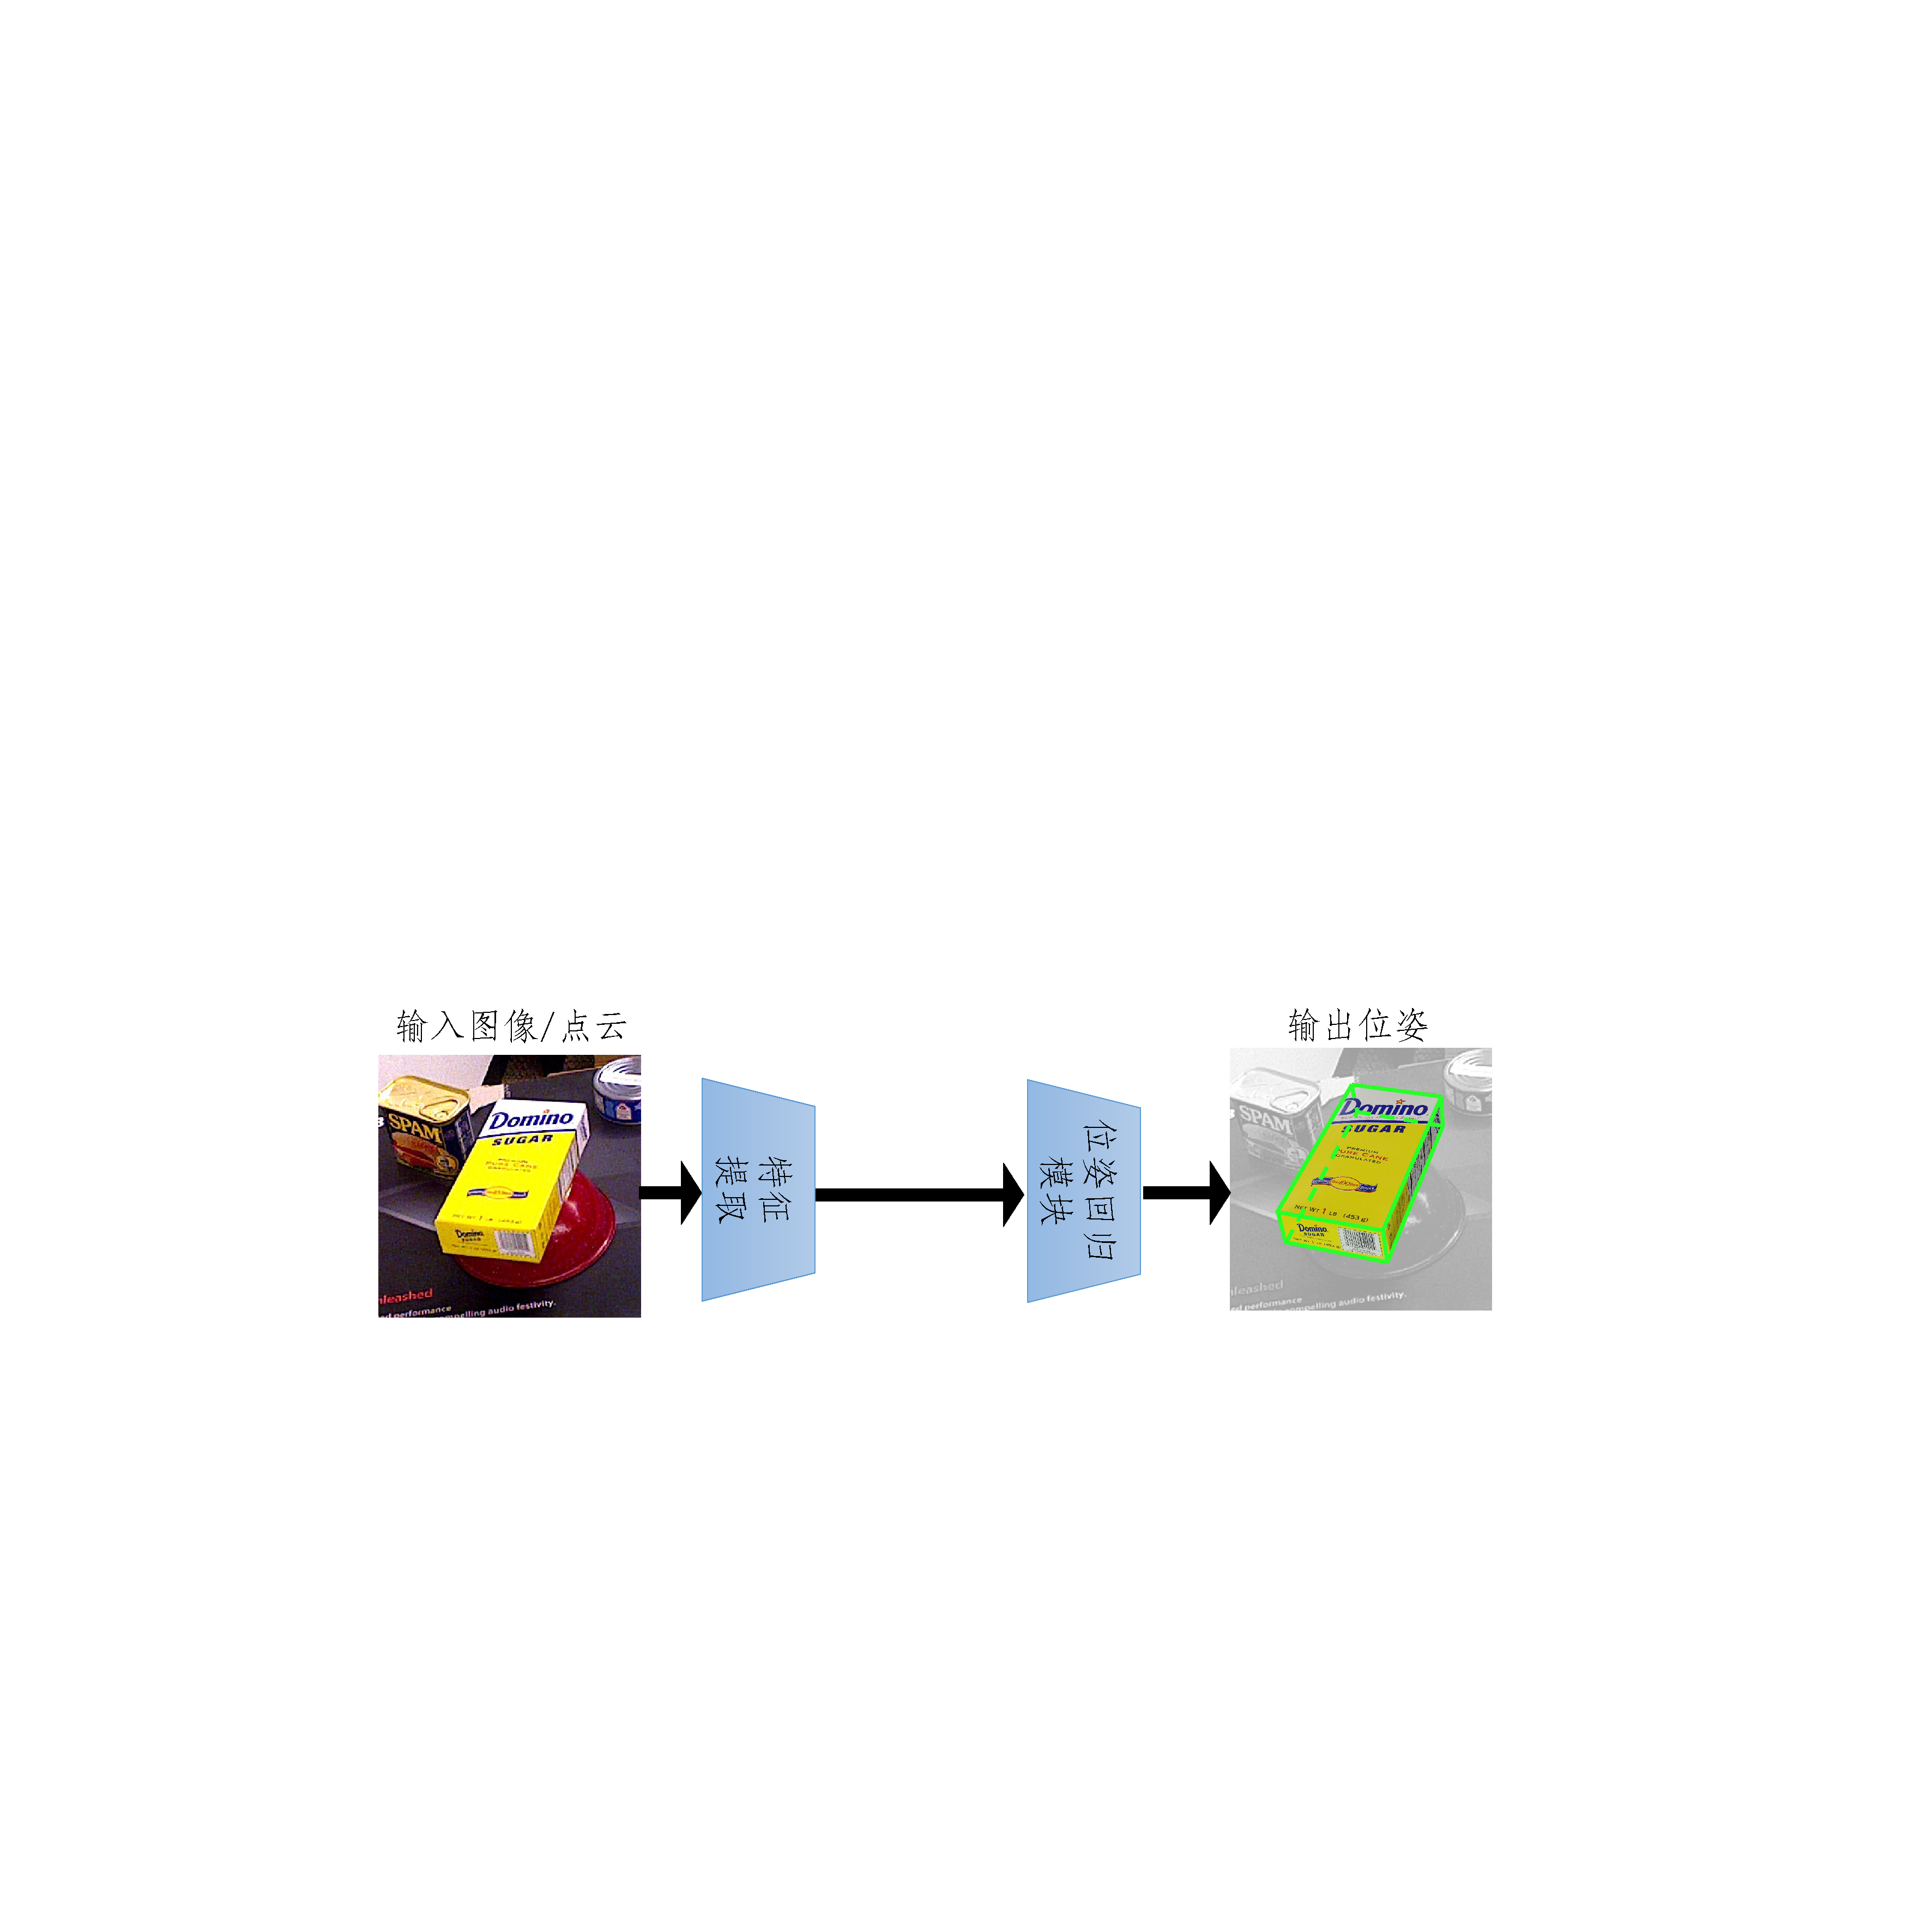
\includegraphics[width=0.95\textwidth]{figure/intro/直接回归法.pdf}
        \caption{直接回归法}
        \label{fig:直接回归法}
    \end{subfigure}
    \vfill
    \begin{subfigure}[b]{0.95\textwidth}
        \centering
        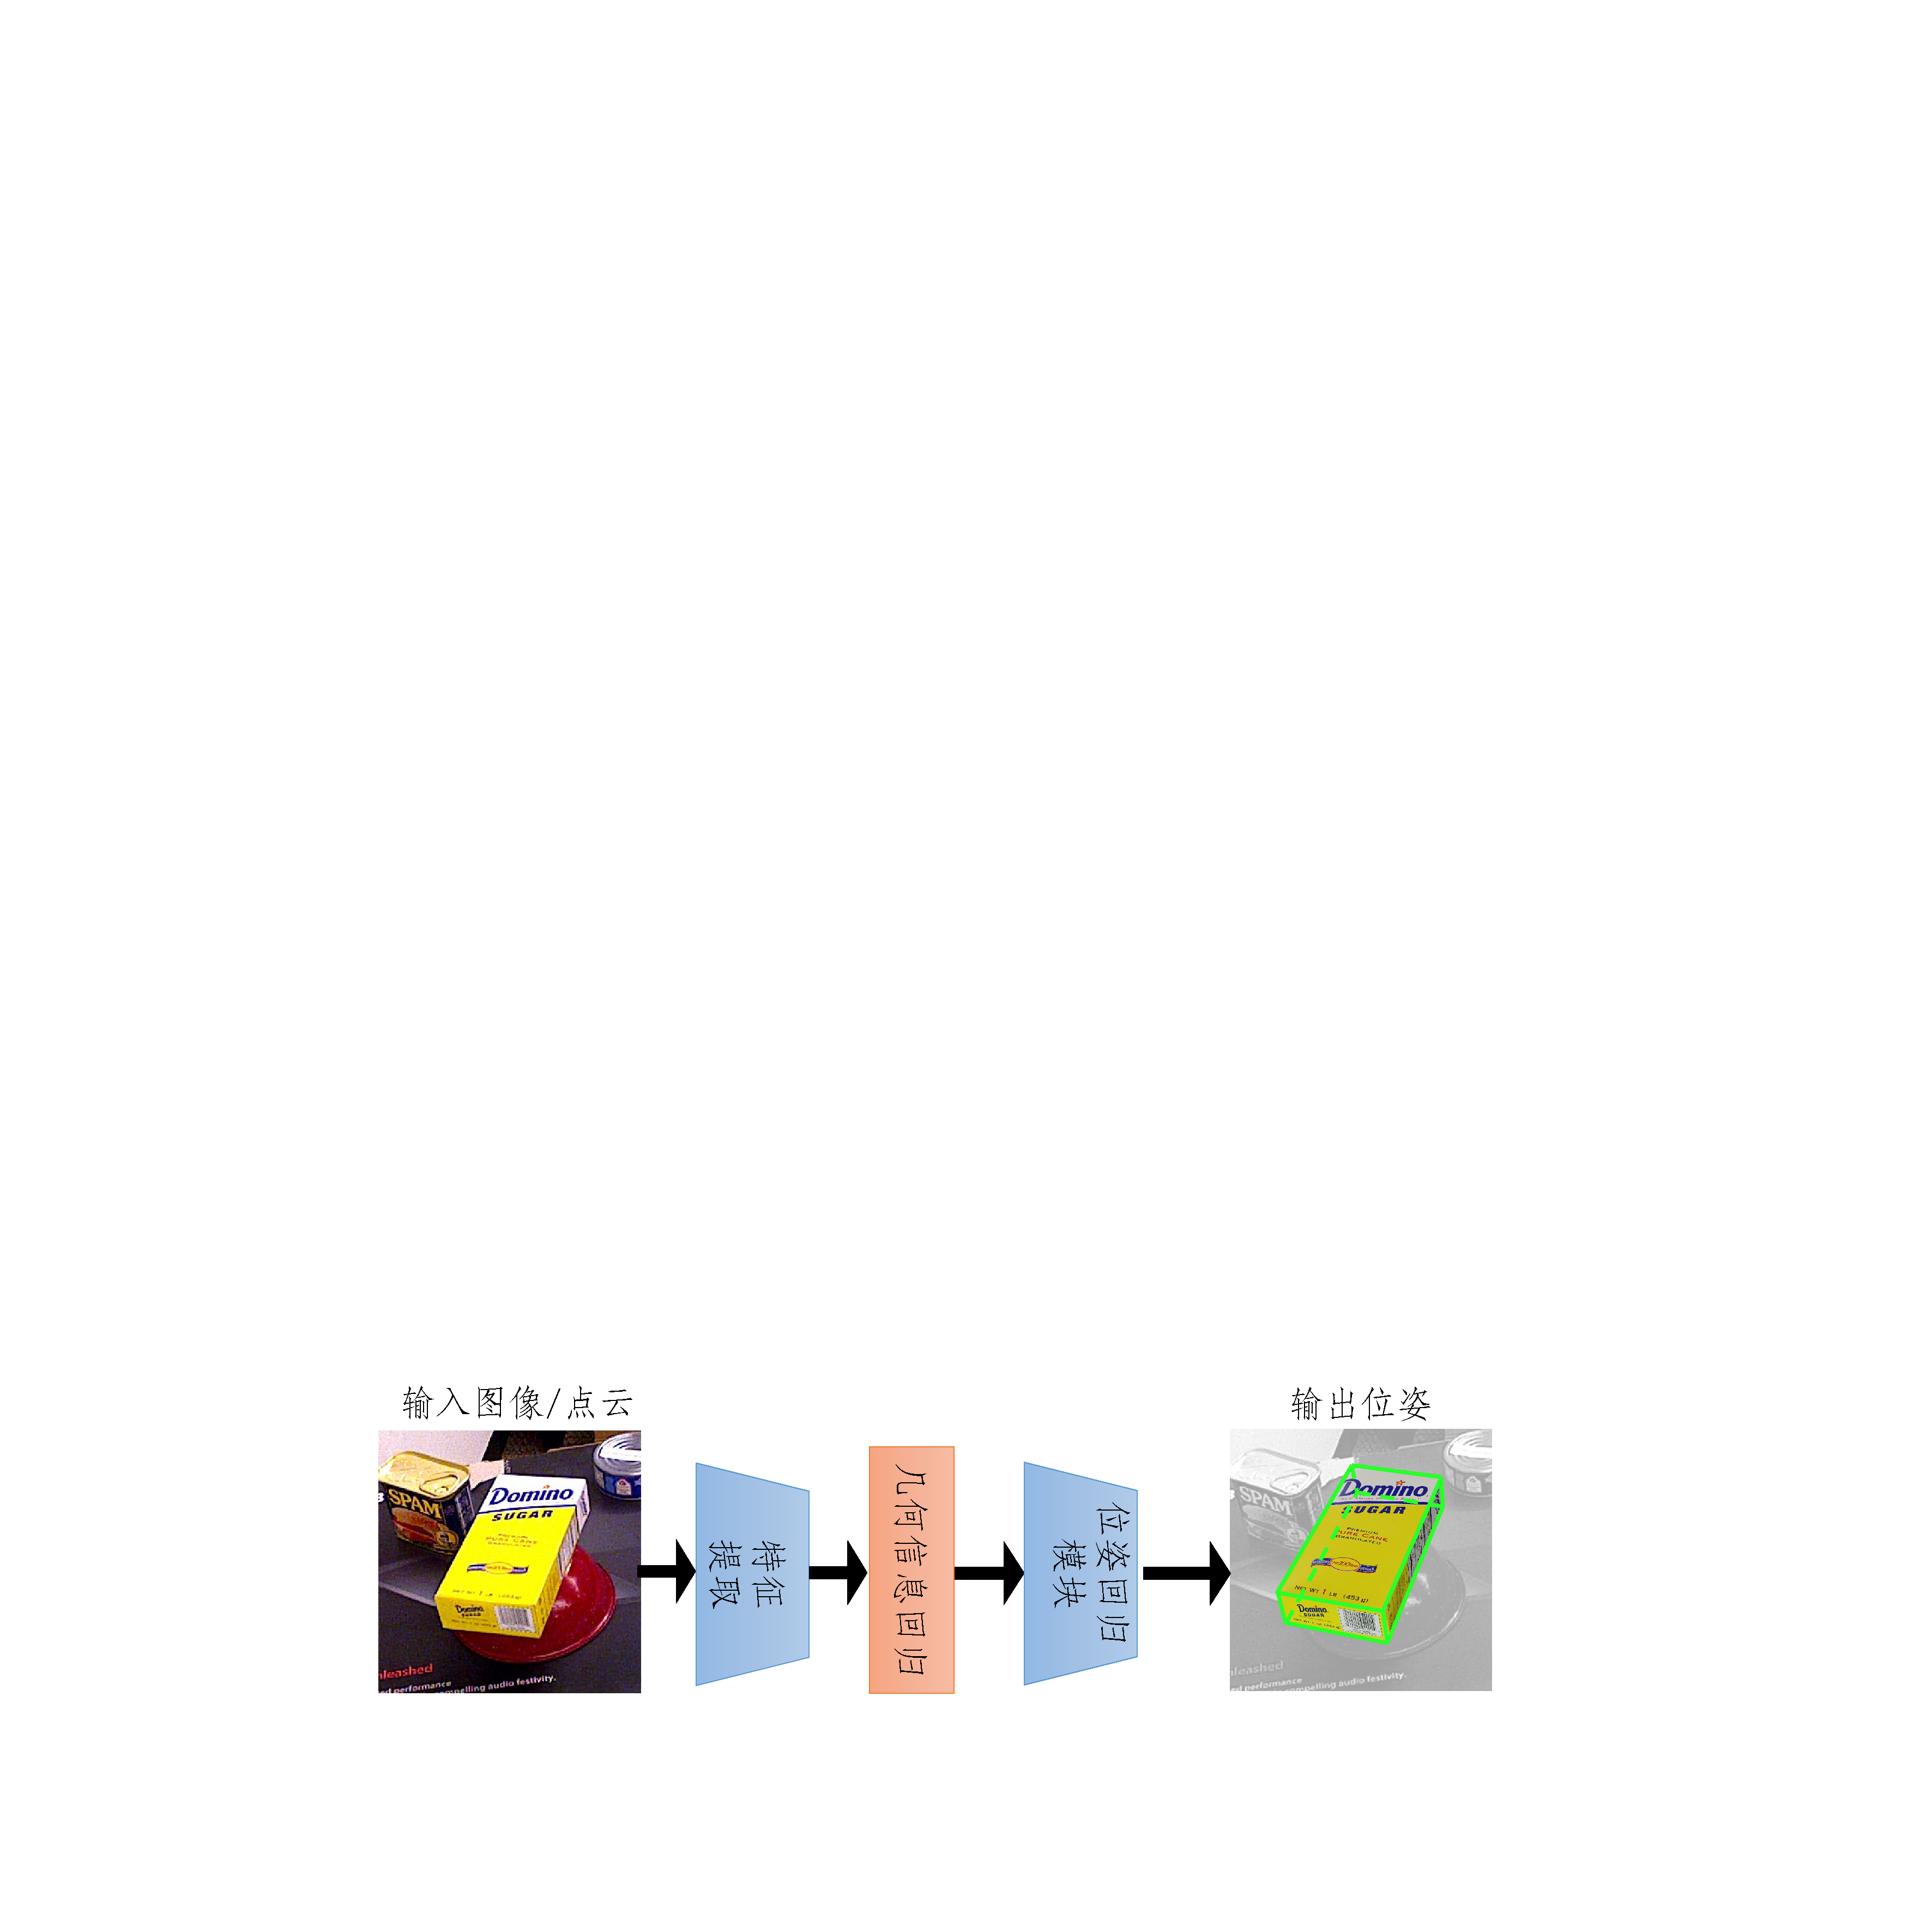
\includegraphics[width=0.95\textwidth]{figure/intro/辅助约束回归方法.pdf}
        \caption{辅助约束回归方法}
        \label{fig:基于辅助约束的回归方法}
    \end{subfigure}
    \caption{基于回归的方法示意图:(a) 直接回归法;(b) 辅助约束回归方法}
    \label{fig:基于回归的方法}
\end{figure}

\subsubsection{直接回归法}\label{直接回归法}

\par SSD-6D\cite{ssd6d}基于SSD检测网络\cite{ssd},首先预测物体的类别和二维边界框,然后对不同拍摄点和在拍摄点绕光轴旋转的角度进行分类。考虑物体的对称性,在数据集收集上,如果物体不具有对称性,则在物体各个角度采集数据集,如果物体具有对称性,只需要在部分区域采集数据。该方法的速度较慢且准确率较低。

\par PoseCNN\cite{ycbv}采用全连接网络输出的三个分支分别为物体类别信息、位置和姿态。对于位置分支,每个像素点都输出物体中心相对当前像素的方向,然后使用霍夫投票的方式找出中心中在图像中的坐标,从而具有一定的对遮挡的鲁棒性,并且回归物体中心的距离相机的距离;对于姿态分支,则直接回归四元数。PoseCNN使用的损失函数是模型在估计姿态中每个点到模型在标注姿态中最近点的平均距离,计算量较大。

\par Deep-6DPose\cite{Deep-6DPose}基于Mask R-CNN网络\cite{maskrcnn},添加了位姿回归网络分支,对于每一个可能包含对象的提案区域(proposal),也称为感兴趣区域(Region of Interest,RoI),都输出一个4维向量,其中3维用李代数表示旋转,还有一维为平移的z轴分量。

\par EfficientPose\cite{bukschat2020efficientpose}基于EfficientNet网络\cite{koonce2021efficientnet},在分类和边界框回归的基础上增加了回归旋转和平移的部分,其损失函数与PoseCNN的损失函数类似。借助EfficientNet网络的轻量化特性和高精度,该方法能够同时输出多个物体的位姿估计,不仅在精度上取得了更好的效果,而且在运行速度上达到了每秒27帧。此外,Wu等人的工作\cite{wu2018real}也采用两个并行的FCN\cite{FCN}分支分别回归物体的旋转和平移参数。此外,Jiang等人\cite{jiang2022uni6d}融合了RGB-D数据、内置的2D像素坐标编码以及深度法向量特征,以更好地估计物体的旋转和平移参数。

\par Tian等人\cite{tian2020robust} 在SO(3)中均匀采样旋转锚点,随后预测每个锚点相对于目标的约束偏差。他们利用不确定性评分选择最佳预测,然后通过聚合点到中心向量检测3D平移,从而估计6D位姿。DenseFusion\cite{wang2019densefusion} 基于逐像素融合RGB和深度特征,并利用姿态预测器为每个像素生成6自由度位姿和置信度。随后,他们选择置信度最高的像素的位姿作为最终位姿。
Zhou等人\cite{zhou2020novel} 使用卷积神经网络提取RGB特征,并将其与点云融合以获得融合特征。与DenseFusion\cite{wang2019densefusion}不同,融合特征以点集形式存在,而非特征映射。
然而,上述RGB-D融合方法仅简单拼接RGB和深度特征,未深入挖掘其内在关系。因此,PR-GCN\cite{Zhou2021PRGCNAD} 提出了一种新的多模态融合图卷积网络,通过局部信息传播捕捉跨模态相关性,从而增强RGB与深度图像的融合。
Liu等人\cite{liu2023depth} 将深度图像中的尺度相关信息和尺度不变信息解耦,引导网络感知场景的3D结构,并为RGB图像特征提取提供场景纹理。与上述使用静态图像的方法不同,TemporalFusion\cite{mu2021temporalfusion} 提出了一种时间融合模型,整合RGB-D图像中的时间运动信息进行6自由度物体位姿估计。该方法能够有效捕捉物体运动和变化,从而提升位姿估计的准确性和稳定性。

\par 为解决物体对称问题,ES6D\cite{mo2022es6d} 设计了一种对称不变的位姿距离度量,使网络能够准确估计对称物体的姿态。SC6D\cite{cai2022sc6d} 引入了3D旋转表示,学习物体的隐式对称性,从而无需额外的对称性先验知识。

\subsubsection{基于辅助约束的回归方法}\label{基于辅助约束的回归方法}

\par \autoref{基于对应关系的方法}中提到的对应关系是一种直观的辅助约束,常被用于辅助约束回归中。

\par SO-Pose\cite{di2021so}提出了一种基于共享编码器和两个独立解码器的方法,用于生成2D-3D对应关系和自遮挡信息,从而提高了物体姿态估计在遮挡情况下的鲁棒性。随后,GDR-Net\cite{wang2021gdr}提出了一种基于几何引导的直接回归网络,通过端到端的方式从密集的2D-3D对应关系中学习物体姿态。Wang等人\cite{wang2021occlusion}进一步引入了噪声增强的学生训练和可微分渲染技术,结合GDR-Net框架\cite{wang2021gdr},通过多几何约束的自监督学习实现了对遮挡场景的鲁棒处理。

\par Trans6d\cite{zhang2022trans6d}则提出了一种基于Transformer的位姿估计方法,该方法包含一个基于图像块(patch)的特征融合模块和一个基于Transformer的优化模块,旨在解决卷积神经网络在捕获全局依赖性方面的局限性。NVR-Net\cite{feng2023nvr}将旋转分解为两组对应的3D法线,这种分解策略显著提高了旋转精度。此外,RNNPose\cite{Xu2024RNNPose} 将物体位姿优化表述为一个非线性最小二乘问题,利用估计的对应关系场,即RGB图像与使用初始位姿渲染的图像之间的对应关系。然后通过可微分的列文伯格-马夸尔特算法\cite{Levenberg_Marquardt}求解非线性最小二乘问题,实现端到端训练。

\par 基于辅助约束的回归方法通过辅助学习其他信息来引导网络学习关键知识,从而提升端到端训练的效果和收敛速度。

\autoref{tab:回归方法}展示了部分代表性方法的属性及性能。在技术方法中,各符号的含义分别为:D 表示目标检测(object detection)、S 表示实例分割(instance segmentation)、V 表示投票(voting)、C 表示对应关系预测(correspondence prediction)、P 表示位姿求解/回归(pose solution/regression)、R 表示位姿优化(pose refinement)。性能指标方面,对于 LM-O 和 LM 数据集,采用物体直径 10\% 范围内(即 ADD(S)-0.1d)的平均召回率作为评价标准;对于 YCB-V 数据集,则采用 ADD-S(<0.1 米)的 AUC 值进行评估。


\begin{table}[!t]
    \centering
    \renewcommand\arraystretch{1}
    \caption{基于回归的方法总结}
    \resizebox{\textwidth}{!}{%
    \begin{tabular}{|ccc|c|c|c|c|c|c|c|c|}
    \hline
    \multicolumn{3}{|c|}{方法} & \begin{tabular}[c]{@{}c@{}}发表\\ 年份\end{tabular} & \begin{tabular}[c]{@{}c@{}}数据\\ 模态\end{tabular} & \begin{tabular}[c]{@{}c@{}}方法\\ 架构\end{tabular} & 创新点 &\multicolumn{2}{l|}{\begin{tabular}[c]{@{}c@{}}LM-O $|$ LM\\ ADD(S)-0.1d\end{tabular}} & \begin{tabular}[c]{@{}c@{}}YCB-V\\ ADD-S ($<$0.1m)\end{tabular} \\ 
    \hline
    
    \multicolumn{1}{|c|}{\multirow{9}{*}{\rotatebox{90}{\centering{基于回归的方法}}}} & \multicolumn{1}{l|}{\multirow{5}{*}{\rotatebox{90}{\centering{直接回归法}}}} & PoseCNN\cite{ycbv} & 2017 & RGB & S+V+P & 杂乱背景 & \multicolumn{1}{c|}{24.9} & - & 75.9 \\
    \cline{3-10} 
    
    \multicolumn{1}{|c|}{} &\multicolumn{1}{l|}{}& Li 等人\cite{li2018unified} & 2018 & RGB-D & P+R & 通用 & \multicolumn{1}{c|}{-} & - & 94.3 \\
    \cline{3-10} 

    \multicolumn{1}{|c|}{} &\multicolumn{1}{l|}{}& Uni6d\cite{jiang2022uni6d} & 2022 & RGB-D & P & 通用 & \multicolumn{1}{c|}{30.8} & 97.0 & 95.2 \\
    \cline{3-10} 

    \multicolumn{1}{|c|}{} &\multicolumn{1}{l|}{}& Hai 等人\cite{hai2023shape} & 2023 & RGB & P & 通用 & \multicolumn{1}{c|}{66.4} & 99.3 & - \\
    \cline{2-10}

    \multicolumn{1}{|c|}{} & \multicolumn{1}{c|}{\multirow{5}{*}{\rotatebox{90}{\centering{辅助约束回归}}}} & GDR-Net\cite{wang2021gdr} & 2021 &  RGB & D+P & 通用 & \multicolumn{1}{c|}{62.2} & - & 91.6 \\
    \cline{3-10} 
    
    \multicolumn{1}{|c|}{} & \multicolumn{1}{l|}{} & SO-Pose\cite{di2021so} & 2021 & RGB & D+C+P & 遮挡 & \multicolumn{1}{c|}{62.32} & 96.0 & 90.9 \\
    \cline{3-10}

    \multicolumn{1}{|c|}{} & \multicolumn{1}{l|}{}& Wang等人\cite{wang2021occlusion} & 2021 & RGB & D+C+P & 遮挡 & \multicolumn{1}{c|}{59.8} & 85.6 & 90.5 \\
    \cline{3-10}

    \multicolumn{1}{|c|}{} &\multicolumn{1}{l|}{}& DGECN\cite{cao2022dgecn} & 2022 & RGB & V+P & 通用 & \multicolumn{1}{c|}{58.7} & - & 90.9 \\
    \cline{3-10}
    
    \multicolumn{1}{|c|}{} & \multicolumn{1}{l|}{} & RNNPose\cite{Xu2024RNNPose} & 2024 & RGB & P+R & 遮挡 & \multicolumn{1}{c|}{60.7} & 97.4 & 85.7 \\

    \hline
    \end{tabular}%
    }
    \label{tab:回归方法}
    \vspace{-1em}
\end{table}

\subsection{基于对比的方法}\label{基于对比的方法}

\par 基于对比的方法可大致分成两类:模板检索和迭代优化,如\autoref{fig:基于对比的方法}。

\par 基于模板检索的方法通过利用图像全局信息,可有效解决无纹理物体带来的挑战。该类方法的核心是从带有真实位姿标注的模板库中检索最相似模板。当输入为RGB图像时,模板库由物体CAD模型投影生成的二维图像及其真实位姿标注构成,此时位姿估计转化为图像检索任务。迭代优化法延续传统方法中迭代匹配的思路,将渲染器得到的初始估计位姿渲染下的图像与输入图像进行对比,得出一个更加优化的估计位姿,重复上述过程最后得到更加精确的估计位姿。该类方法往往用于后处理,提升其他方法的最终性能。

\begin{figure}[htbp]
    \centering
    \begin{subfigure}[b]{0.95\textwidth}
        \centering
        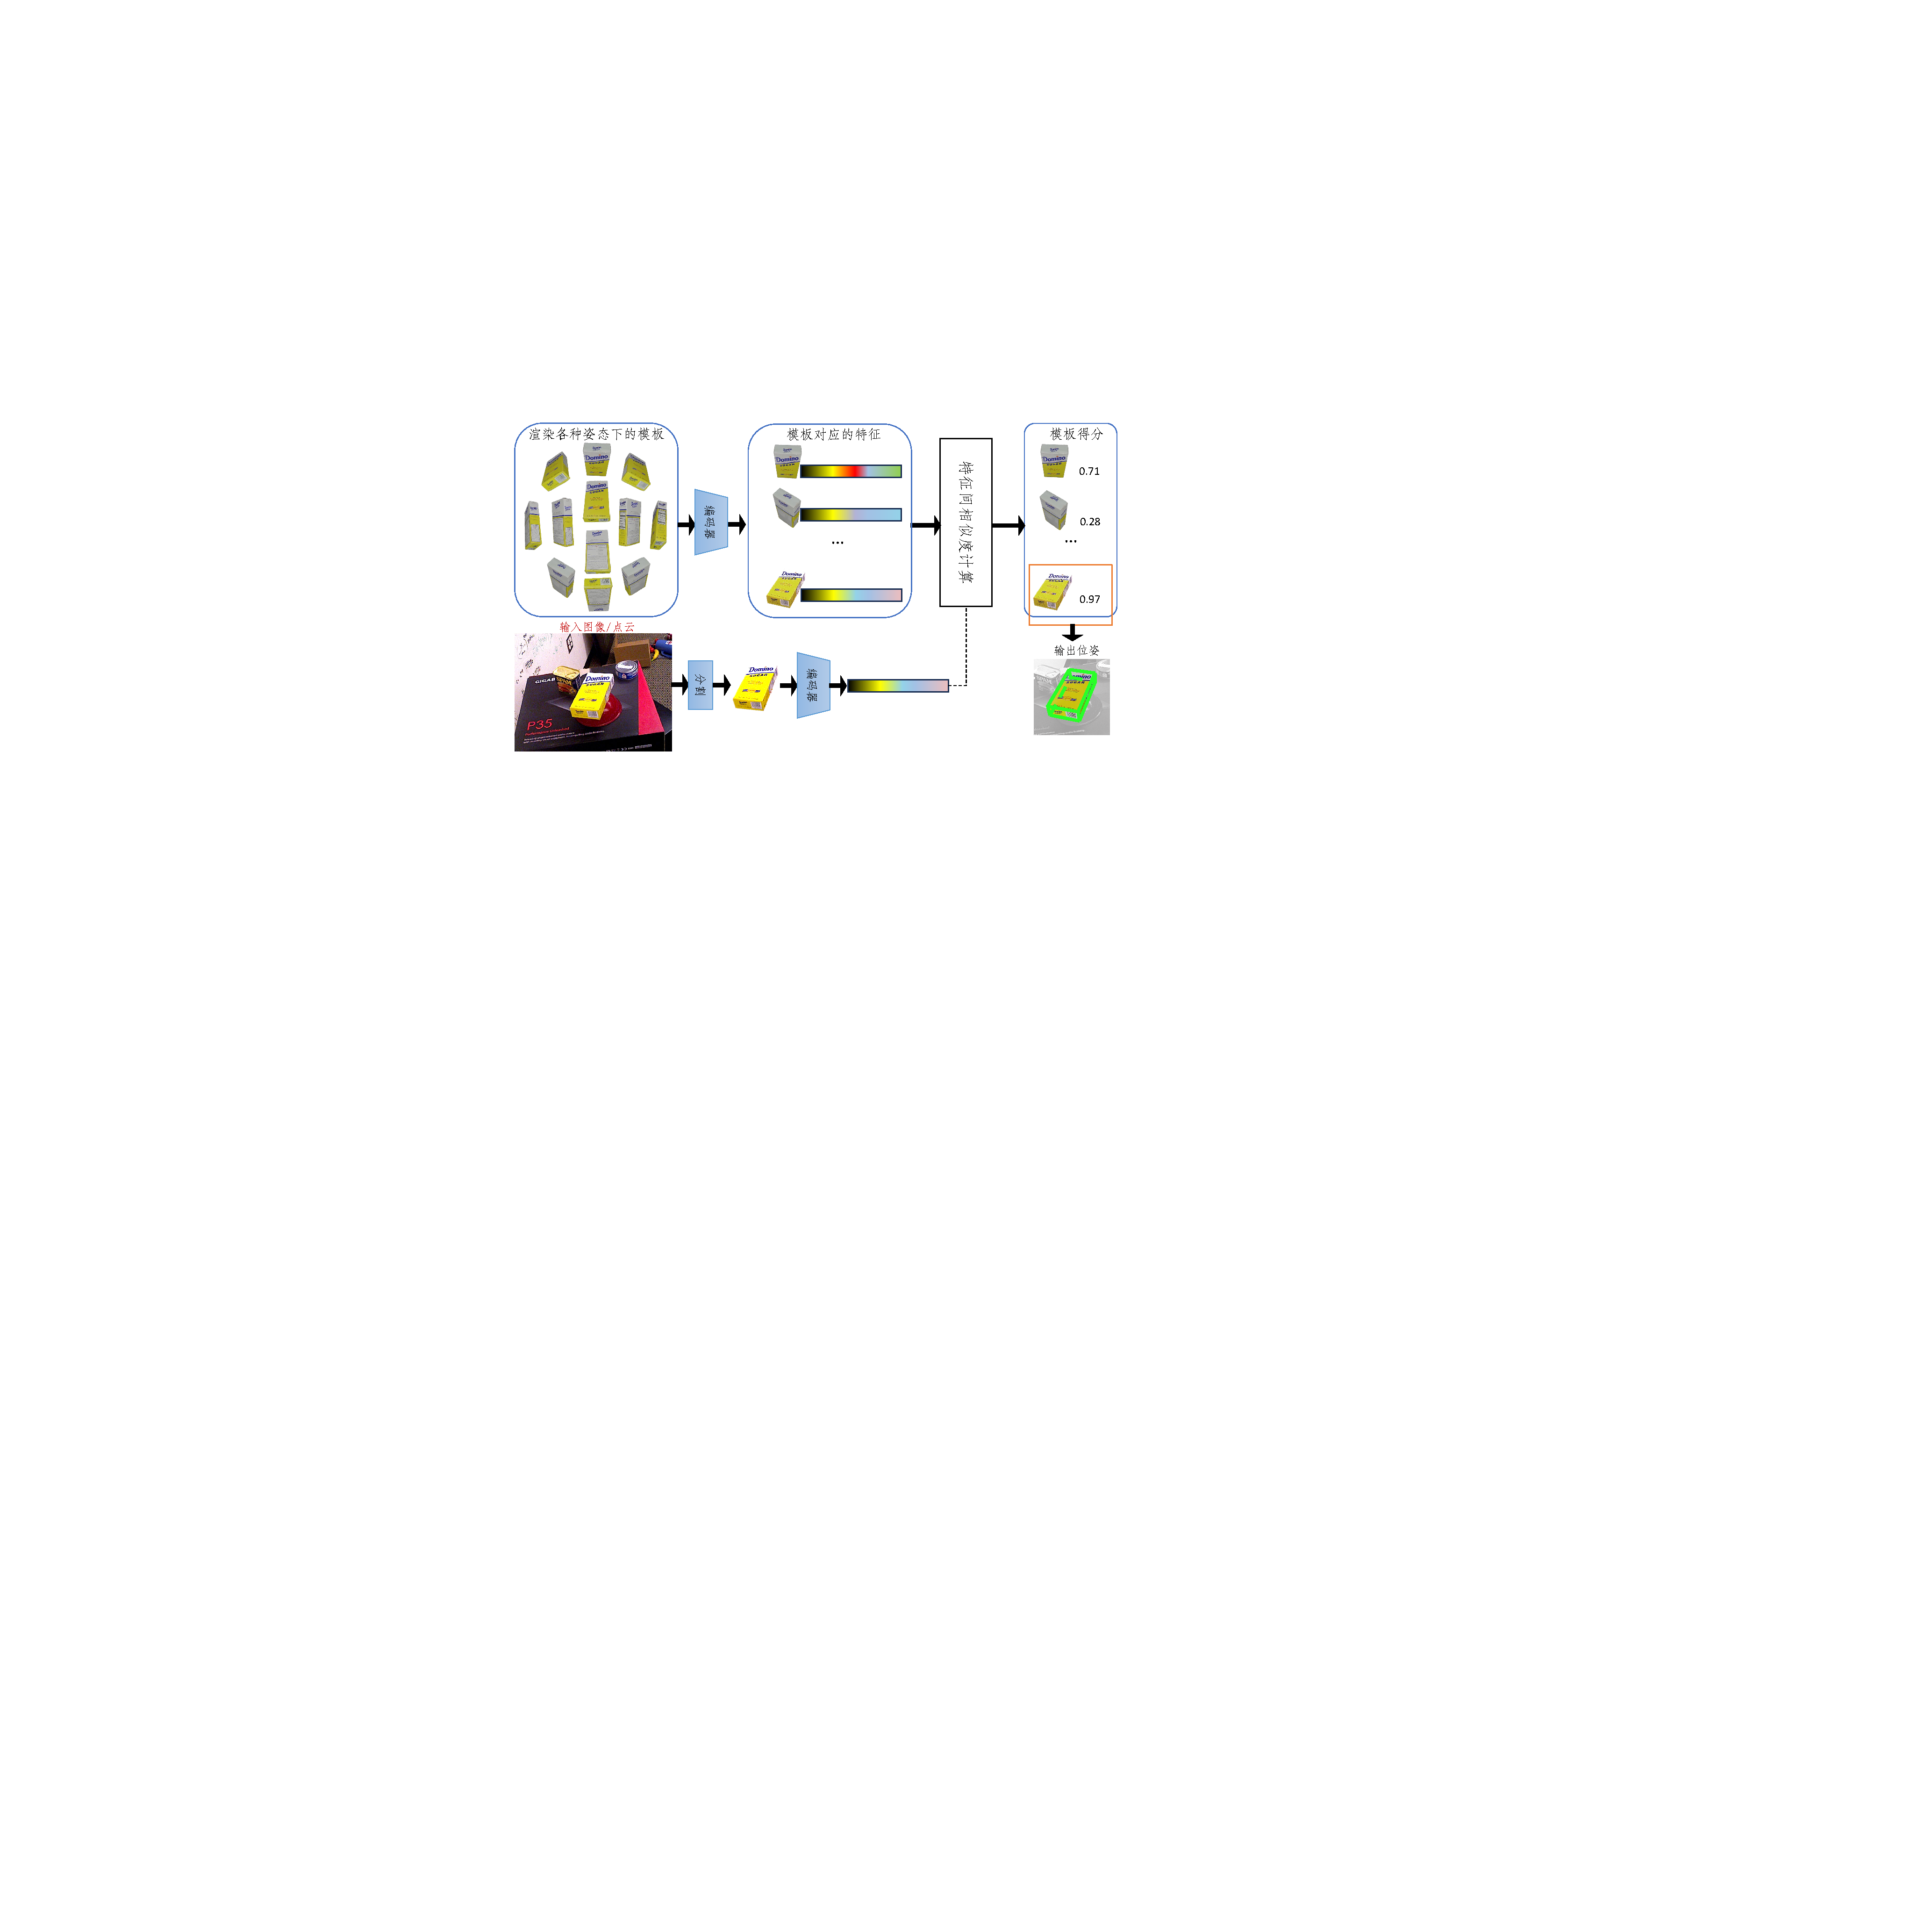
\includegraphics[width=0.95\textwidth]{figure/intro/模板检索.pdf}
        \caption{基于模板检索的方法}
        \label{fig:基于模板检索的方法}
    \end{subfigure}
    \vfill
    \begin{subfigure}[b]{0.95\textwidth}
        \centering
        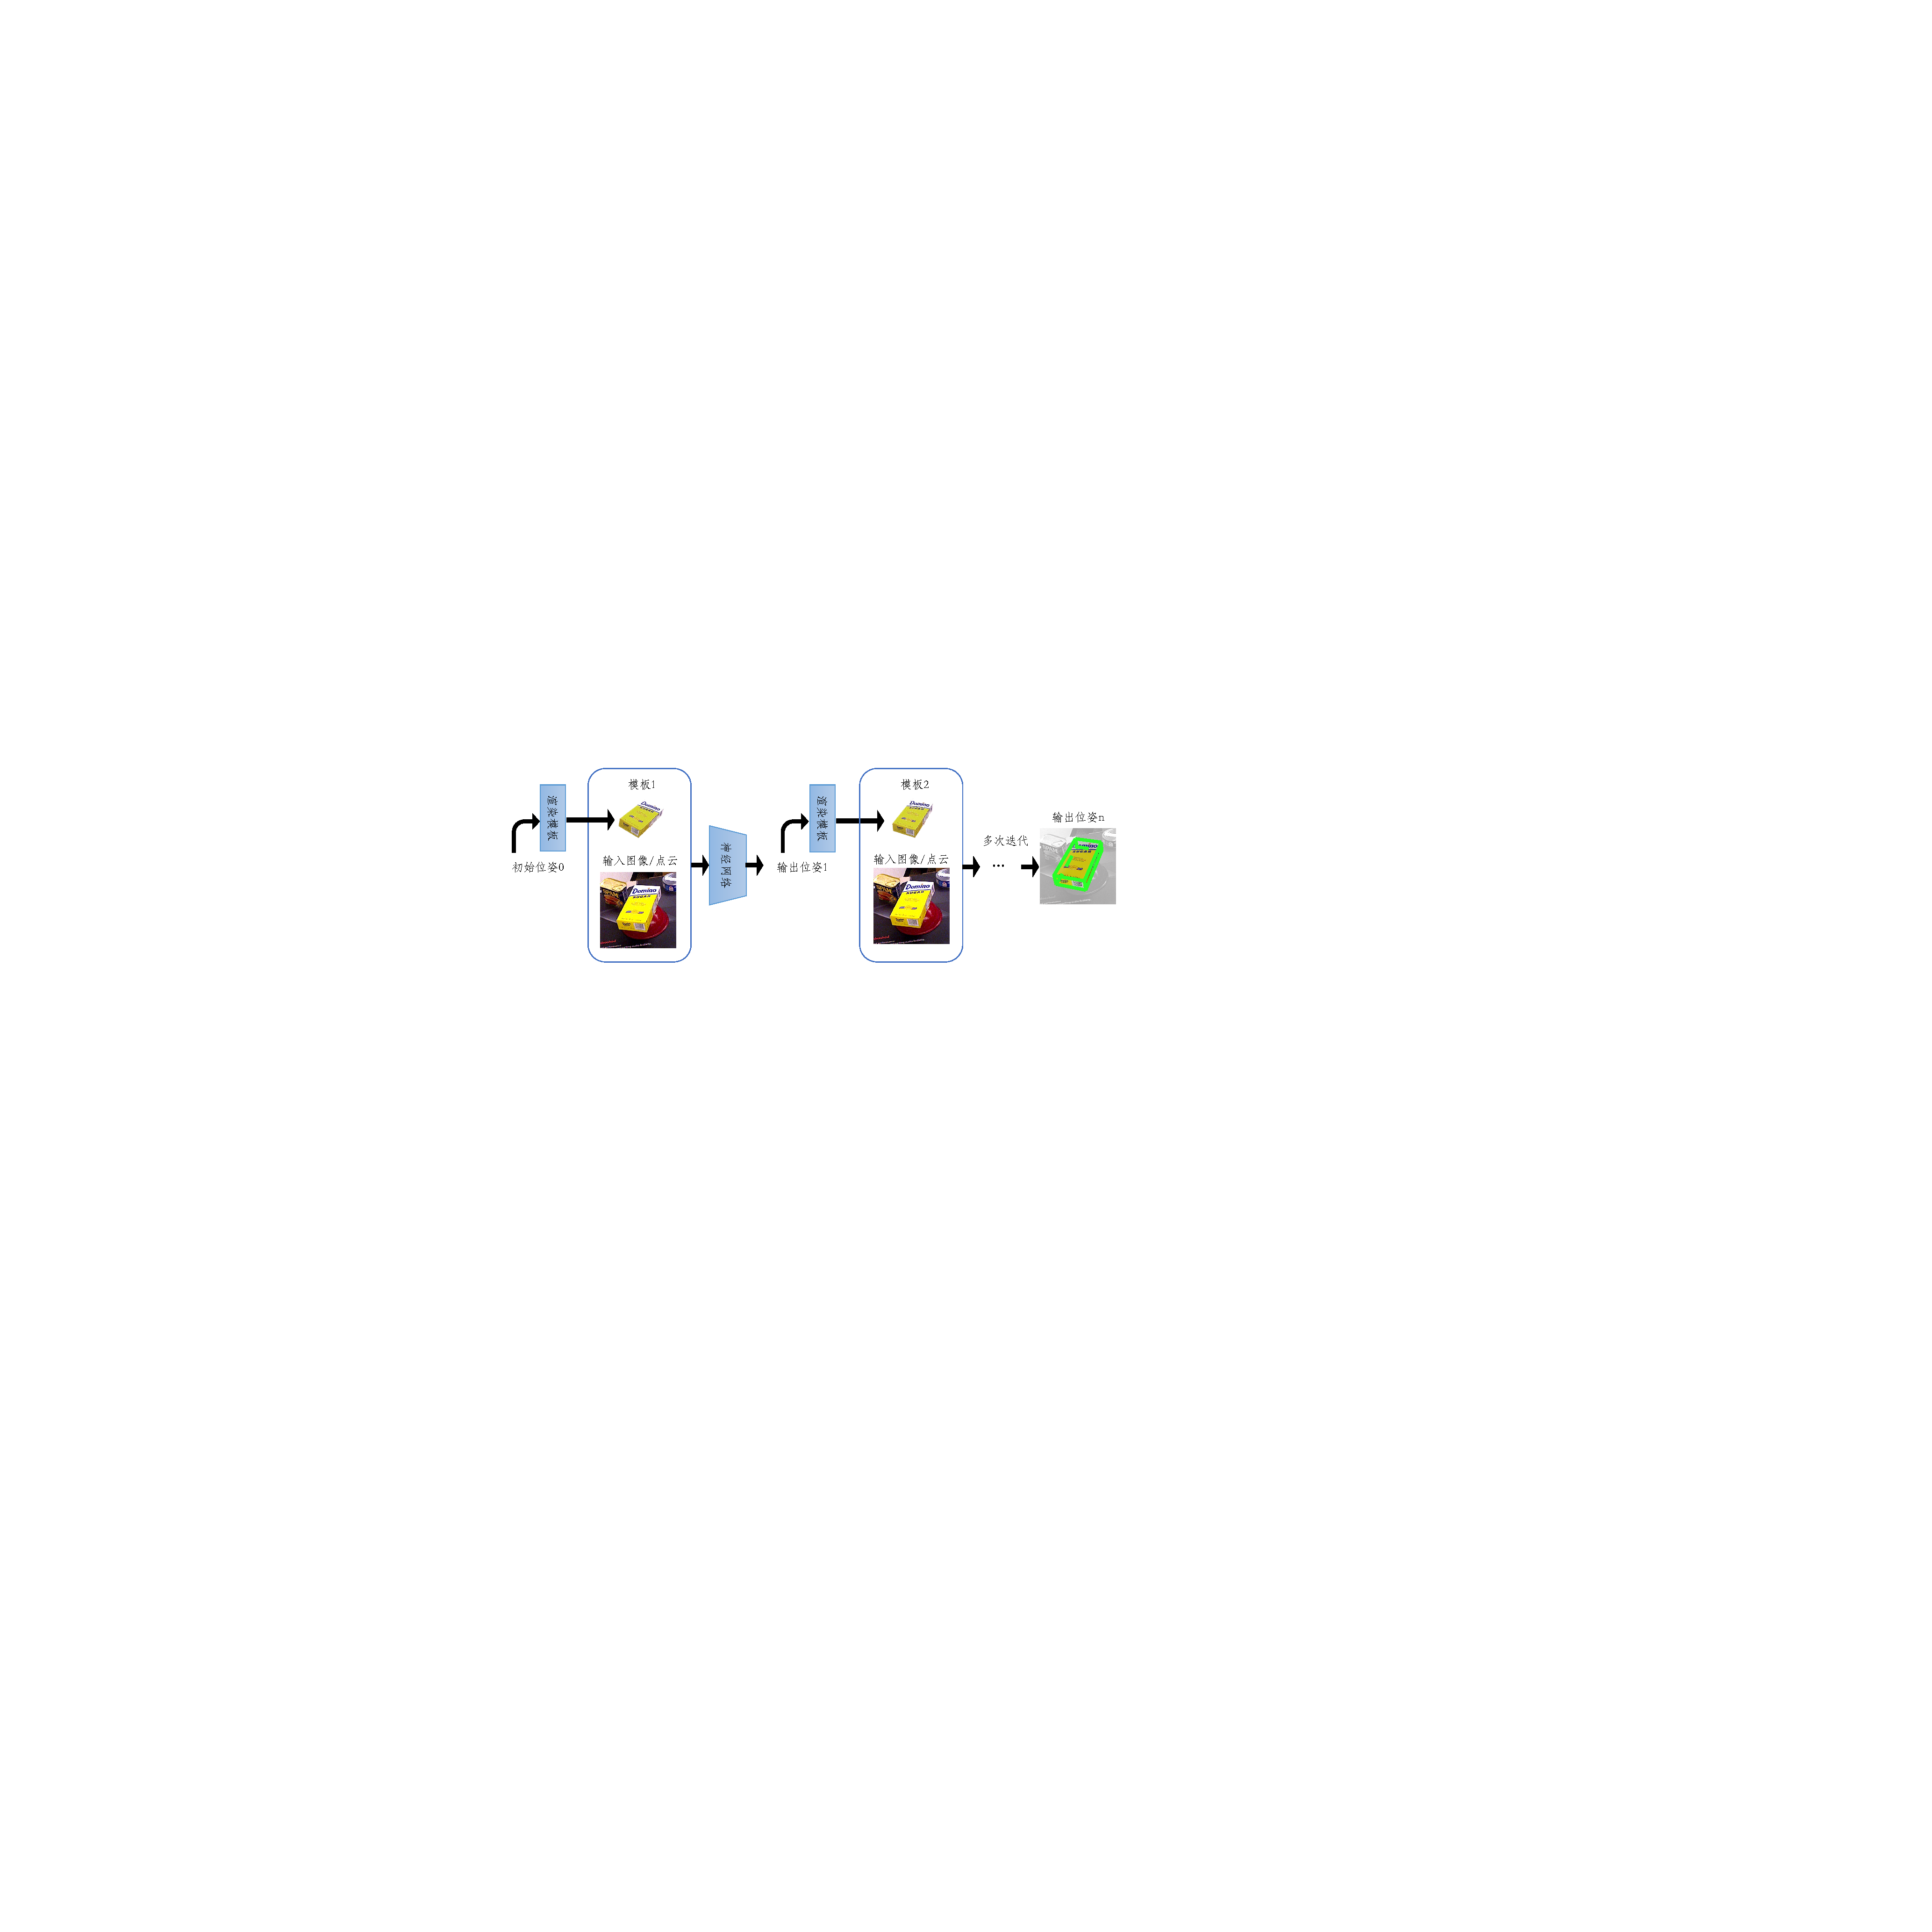
\includegraphics[width=0.95\textwidth]{figure/intro/迭代优化.pdf}
        \caption{基于迭代优化的方法}
        \label{fig:基于迭代优化的方法}
    \end{subfigure}
    \caption{基于对比的方法示意图:(a) 模板检索法;(b) 迭代优化法}
    \label{fig:基于对比的方法}
\end{figure}

\subsubsection{基于模板检索的方法}\label{基于模板检索的方法}

\par AAE(Augmented Autoencoder)\cite{sundermeyer2018implicit}使用域随机化(Domain Randomization)生成不同状态(不同位置、不同姿态、不同纹理、不同遮挡、不同光照等)下的输入图像,训练增强自编码器编码位姿相关的特征,且能够忽略其他状态的影响。训练完成后将各个视角下渲染的模型图像输入AAE网络中,输出对应的隐式表示向量,存储为编码本。在测试时,将输入图像输入AAE网络后输出对应的隐式表示向量,与编码本中的向量一一比较余弦相似度,选出其中相似度最高的编码对应的姿态作为预测姿态。

\par Liu等人\cite{Liu2019cutout}开发了一种类似于自动编码器的卷积神经网络,用于重建包含目标物体的任意场景并提取物体区域。此外,Zhang等人\cite{Zhang2020preprocessing}利用目标检测器和关键点提取器来简化模板搜索过程。

\par Papaioannidis等人\cite{9206072}指出,在合成图像中估计物体姿态更为直接。因此,他们采用了生成对抗网络,将真实图像转换为合成图像,同时保留物体的姿态。Li等人\cite{Li2020Pose}使用了一种新的姿态表示方法,3D位置场,引导自动编码器提炼与姿态相关的信息,从而提高了处理姿态的能力。Stev\v{s}i\v{c}等人\cite{Stev2020Spatial}提出了一种空间注意力机制,用于识别和利用空间细节进行姿态优化。与上述方法不同,PoseRBPF\cite{Deng2021PoseRBPF}在 Rao-Blackwellized 粒子滤波框架\cite{Murphy2001}下解决了6自由度物体位姿跟踪问题。他们对旋转空间进行了精细的离散化处理,并训练了一个自动编码器网络,为这些离散化的旋转构建了一个特征编码本。该方法能够高效地估计3D平移以及完整的3D旋转分布。

\par 基于模板检索的方法通过从带有真实位姿标注的模板库中检索最相似模板来估计物体位姿,其精度依赖于模板数量,且对遮挡的处理能力有限。

\subsubsection{基于迭代优化的方法}\label{基于迭代优化的方法}

DeepIM\cite{li2018deepim}首先利用目标检测算法得到目标物体在输入图像中的区域,同时用初始估计位姿对三维模型进行渲染,得到渲染的图片。将两张图片及对应物体区域的掩码输入网络,网络输出位姿估计的修正量。为了提升训练的稳定性,在训练阶段和额外增加光流分支和掩码分支。光流分支根据两张输入的图片得到两者的光流信息,掩码分支给出输入图片的掩码。DeepIM网络架构基于FlowNet\cite{dosovitskiy2015flownet},输出3维的平移向量和4维的四元数。

\par CosyPose\cite{labbe2020cosypose}在DeepIM\cite{li2018deepim}的基础上进行改进,提高单目6D位姿估计的精度。其骨干网络不使用FlowNet\cite{dosovitskiy2015flownet}而改用EfficientNet-B3\cite{koonce2021efficientnet},并且不使用辅助训练分支。旋转表示不使用四元数而使用旋转矩阵的前两行,使用更好的深度和平移预测的损失函数。同时,为了提高网络的适用性,输入网络的焦距根据对图像的操作也会调整。根据实验结果,CosyPose能够实现效果大幅提升主要依赖于利用提供的CAD模型生成百万张照片进行训练。CosyPose使用了替换背景、图像调色、加入噪声等的数据增广来生成更多的训练数据,训练更具有泛化能力的网络。

\par Manhardt 等人\cite{manhardt2018deep}通过对比RGB图像与渲染轮廓之间的物体轮廓,优化了6D位姿。渲染轮廓是通过初始位姿从物体CAD模型中获得的。Hai 等人\cite{hai2023shape}提出了一种基于形状约束的递归匹配框架来优化初始位姿。他们首先基于初始位姿和当前估计的位姿计算诱导的光流,然后直接从诱导的光流中解耦6自由度的位姿。

\par 为了解决位姿优化方法运行效率低的问题,RePOSE\cite{iwase2021repose}引入了一种基于深度纹理渲染的位姿优化方法,利用具有可学习纹理的物体CAD模型进行快速特征提取。MRC-Net\cite{li2024mrcnet}提出了一种两阶段方法。第一阶段进行位姿分类,并在分类的位姿下渲染物体CAD模型。第二阶段进行回归,预测分类位姿下的精细残差。该方法通过位姿分类引导残差位姿回归,从而提高了鲁棒性。

一些研究者专注于仅回归3D旋转,以实现更高效和实用的位姿估计。Papaioannidis 等人\cite{8765585}提出了一种基于四元数的多目标损失函数,将流形学习与回归相结合,用于学习3自由度的姿态描述符。他们通过回归学习到的描述符获得了3自由度的姿态。Liu 等人\cite{liu2019regression}基于卷积神经网络训练了一个三重网络,从二值图像中提取判别性特征。他们在构建的三重网络中引入了姿态引导方法和回归约束,使特征适应回归任务,从而增强了鲁棒性。

\begin{table}[thbp]
    \centering
    \renewcommand\arraystretch{1}
    \caption{基于对比的方法总结}
    \resizebox{\textwidth}{!}{%
    \begin{tabular}{|ccc|c|c|c|c|c|c|c|c|}
    \hline
    \multicolumn{3}{|c|}{方法} & \begin{tabular}[c]{@{}c@{}}发表\\ 年份\end{tabular} & \begin{tabular}[c]{@{}c@{}}数据\\ 模态\end{tabular} & \begin{tabular}[c]{@{}c@{}}方法\\ 架构\end{tabular} & 创新点 &\multicolumn{2}{l|}{\begin{tabular}[c]{@{}c@{}}LM-O $|$ LM\\ ADD(S)-0.1d\end{tabular}} & \begin{tabular}[c]{@{}c@{}}YCB-V\\ ADD-S ($<$0.1m)\end{tabular} \\ 
    \hline
    
    \multicolumn{1}{|c|}{\multirow{9}{*}{\rotatebox{90}{\centering{基于对比的方法}}}} & \multicolumn{1}{l|}{\multirow{4}{*}{\rotatebox{90}{\centering{模板}}}} & AAE\cite{sundermeyer2018implicit} & 2018 & RGB & D+T & \begin{tabular}[c]{@{}c@{}}通用\\ 泛化\end{tabular} & \multicolumn{1}{c|}{-} & 31.4 & - \\
    \cline{3-10} 

    \multicolumn{1}{|c|}{} & \multicolumn{1}{l|}{} & Papaioannidis 等人\cite{9206072} & 2020 & RGB & D+T & 通用 & \multicolumn{1}{c|}{-} & - & - \\
    \cline{3-10}

    \multicolumn{1}{|c|}{} & \multicolumn{1}{l|}{} & PoseRBPF\cite{Deng2021PoseRBPF} & 2021 & RGB & D+T & 对称物体& \multicolumn{1}{c|}{-} & - & - \\
    \cline{2-10} 

    \multicolumn{1}{|c|}{} & \multicolumn{1}{c|}{\multirow{6}{*}{\rotatebox{90}{\centering{迭代优化}}}} & DeepIM\cite{li2018deepim} & 2018 & RGB & T+P+R & 通用 & \multicolumn{1}{c|}{55.5} & 88.6 & 81.9 \\ 
    \cline{3-10} 
    
    \multicolumn{1}{|c|}{} &\multicolumn{1}{l|}{}& CosyPose\cite{labbe2020cosypose} & 2020 & RGB & D+T+P+R & \begin{tabular}[c]{@{}c@{}}通用\\ 泛化\end{tabular} & \multicolumn{1}{c|}{-} & - & 93.4 \\ 
    \cline{3-10}

    \multicolumn{1}{|c|}{} & \multicolumn{1}{l|}{}& Wang等人\cite{wang2021occlusion} & 2021 & RGB & D+T+P & 遮挡 & \multicolumn{1}{c|}{59.8} & 85.6 & 90.5 \\
    \cline{3-10}

    \multicolumn{1}{|c|}{} &\multicolumn{1}{l|}{}& Hai 等人\cite{hai2023shape} & 2023 & RGB & T+P+R & 通用 & \multicolumn{1}{c|}{66.4} & 99.3 & - \\
    \cline{3-10}

    \multicolumn{1}{|c|}{} &\multicolumn{1}{l|}{}& MRC-Net\cite{li2024mrcnet} & 2024 & RGB & S+T+P & 通用 & \multicolumn{1}{c|}{-} & - & 97.0 \\

    \hline
    \end{tabular}%
    }
    \label{tab:渲染方法}
    \vspace{-1em}
\end{table}

\autoref{tab:渲染方法}展示了基于对比的方法的部分代表性方法的属性及性能。在方法架构中,各符号含义如下:D、S、T、P、R 分别表示目标检测(object detection)、实例分割(instance segmentation)、模板(template)、位姿求解/回归(pose solution/regression)及位姿优化(pose refinement)。性能指标方面,对于 LM-O 和 LM 数据集,采用物体直径 10\% 范围内(即 ADD(S)-0.1d)的平均召回率作为评价标准;对于 YCB-V 数据集,则采用 ADD-S(<0.1 米)的 AUC 值进行评估。

\section{研究内容与贡献}
\par 本文聚焦于实例级物体位姿估计任务,针对 RGB 数据输入与 RGB-D 数据输入两种典型场景展开深入研究。尽管现有方法在精度上取得了显著进展,但在处理遮挡场景鲁棒性、对称性歧义以及高效优化方法等方面仍存在不足。本文提出了一系列创新方法,包括层次化二进制表面编码使用策略、跨模态特征融合机制、对称感知的表面编码以及基于轮廓对齐的优化策略。通过这些改进,旨在提升位姿估计的精度、鲁棒性和计算效率,为机器人抓取和智能制造等实际应用提供更可靠的技术支持。
\par 针对 RGB-D数据输入场景,重点探究对应关系的表征与应用:通过改进观测点与物体表面区域的对应关系建模方法,降低稠密对应关系的错误匹配;同时设计跨模态特征融合机制,实现RGB色彩信息与深度几何信息的特征融合的效果提升。
\par 针对 RGB数据输入场景,研究内容分为两个递进方向:首先提出面向对称性歧义物体的端到端位姿估计框架,通过设计考虑对称性的稠密对应关系表征,消除姿态解算中的歧义性问题;进一步开发基于边缘特征的精细化优化策略,利用物体轮廓的几何先验知识,在初始估计基础上实现亚像素级精度提升。
\par 本文的核心贡献体现在对实例级物体位姿估计方法的系统性改进与创新,特别是在处理RGB-D与RGB数据输入的场景下,提出了一系列在精度与效率上均达到国际领先水平的算法。具体而言,本文在以下两个关键方面为该领域提供了具有重要影响力的解决方案:
\par \textbf{对应关系的高效利用}:针对RGB-D数据输入场景,本文提出了一种层次化表面编码与对应关系剪枝的创新方法,显著提升了位姿估计的计算效率与匹配精度。通过多尺度特征表征与动态优化策略,有效解决了传统稠密对应方法在计算复杂度与匹配准确性之间的权衡问题。
\par \textbf{对称性歧义的突破}:在仅使用RGB数据输入的场景下,本文提出了一种端到端的位姿估计框架,特别针对具有对称性歧义的物体,通过引入几何对称性约束,有效消除了多义性问题,显著提升了位姿估计的鲁棒性与准确性。
\par 这些成果不仅为物体位姿估计领域提供了新的研究视角与技术路径,也为相关应用如机器人抓取、增强现实等的实际落地提供了坚实的理论与方法支撑。

\section{本文组织架构}

\par 根据研究内容,本文共分为六个章节,\autoref{fig:本文组织架构}展示了本文的组织结构,各章节的内容安排如下:

\begin{figure}[htbp]
    \centering
    \begin{overpic}[width=0.95\textwidth]{figure/intro/本文组织架构.pdf}
    \end{overpic}
    \caption{本文组织架构}
    \label{fig:本文组织架构}
\end{figure}

\par 本文第一章为绪论部分。首先从理论价值与工程应用双重维度,系统性地论述物体位姿估计技术的研究意义及其在智能制造、机器人自主操作等领域的实践价值,通过宏观视角梳理技术演进路线与研究框架,为读者构建基础认知体系。进而回顾国内外在该领域的关键研究成果,着重对比分析不同技术流派的演进脉络与创新突破。本章结尾系统阐释全文的章节架构与内容布局,通过可视化结构示意图清晰展现各章节间的逻辑关联与递进关系,为后续研究内容的展开奠定系统化认知基础。

\par 第二章提出了一种基于单张 RGB-D 图像的实例级物体6D 物体位姿估计方法。该章设计了名为 HiPose 的创新性架构,其核心为层次化表面编码与对应关系剪枝机制。该方法通过多尺度二进制编码策略,从粗到精逐步建立观测点云与物体表面区域的对应关系:首先利用大尺度表面区域进行初始匹配以降低计算复杂度,随后通过迭代优化不断收缩匹配区域,逐步将表面对应关系收敛至精确点对点匹配。HiPose 采用点到表面匹配范式,在迭代过程中同步实施离群点动态剔除,从而在保证位姿精度的同时显著提升算法效率。

\par 第三章提出另一种基于单张RGB-D图像的实例级物体6D 物体位姿估计方法,重点解决RGB外观信息与深度几何信息的高效融合问题。相较于第二章的网络架构,本章的核心创新在双向一致性融合网络的基础上,通过双分支协同学习机制充分挖掘多模态数据的互补性。具体而言,该方法设计了并行的RGB分支与深度分支,分别提取图像表观特征与几何结构特征,弥补了此前工作中对RGB信息利用不足的缺陷。针对双分支网络的优化,提出像素-观测点联合损失函数:在RGB分支中引入像素级特征对齐损失,强化局部纹理一致性;在深度分支中构建顶点级几何约束,确保三维空间匹配精度。此外,通过设计跨模态一致性损失函数,约束两个分支在特征空间与位姿预测结果上的一致性,有效提升网络收敛速度。

\par 第四章提出一种从单张RGB图像中估计物体的6D位姿的方法,这一任务在处理对称物体时更具挑战性。传统方法通常在图像像素与3D物体表面观测点之间建立一对一的对应关系,但这种做法在对称物体上引入了歧义性。为了解决这一问题,提出了一种对称感知的表面编码SymCode。SymCode基于一对多的对应关系对物体表面顶点进行编码,有效消除了单一对应关系带来的歧义问题。此外,还引入了一个高效的端到端深度学习网络SymNet。SymNet能够直接回归6D位姿参数,而无需通过PnP问题进行求解,从而显著提升了位姿估计的效率与准确性。

\par 第五章提出一种基于轮廓对齐的物体位姿优化方法。该方法的核心创新在于通过可见掩码与完整掩码提取感兴趣轮廓 ,并基于此与初始位姿渲染轮廓的几何一致性建立优化目标。具体而言,通过将实际观测轮廓与当前位姿的渲染轮廓进行对齐,构建轮廓匹配误差函数,利用其梯度迭代优化位姿参数。与传统依赖图像渲染与像素级比较的方法不同,本方法仅需渲染物体分割轮廓,无需引入额外的优化网络训练过程,从而显著降低了计算复杂度。这种轻量化设计使位姿优化过程摆脱了对高维特征匹配的依赖,在保证精度的同时实现准确率的提升。

\par 第六章对本文的研究内容进行了总结,并对未来的研究方向进行了展望。


% \par 6自由度物体位姿估计问题是指通过传感器数据计算物体坐标系相对于相机坐标系的位姿变换。位姿变换包括平移分量和旋转分量,能用一个 $4\times 4$ 的位姿变换矩阵描述。传感器数据通常包括单目RGB相机、深度相机或者多目RGB相机或者多个视角的相机组合。物体坐标系和相机坐标系分别定义在物体的模型和相机上。物体的模型通常是一个三维模型,可以是点云、网格(mesh)模型或者CAD模型,通常具有纹理或颜色信息。相机的模型通常是一个消除了畸变的针孔相机模型,相机内参 $K$ 已知。

% \par 刚性物体在空间中的位置和姿态具有六个自由度(6 Degree of Freedom,又称6DoF或6D),其中三个平移自由度,用笛卡尔坐标系中的坐标表示;三个旋转自由度,可以用欧拉角、四元数、旋转矩阵等方式进行表示。物体的6D位姿估计就是通过传感器获取场景图像、点云等信息,最终获得场景中目标物体在相机坐标系或者世界坐标系下的位置和姿态。

% \par 目标物体的位姿估计问题是一个视觉感知问题,是机器人应用中重要的基础问题。只有机器人系统实现目标物体的定位,才能够实现环境交互,例如机械臂实现物体抓取、物体操作以及避障和跟踪等下游任务。目前,操作机器人还无法广泛应用于非工业场景,主要原因便是对于环境理解的能力不足,无法快速适应非结构化甚至未知环境。因此,解决位姿估计问题能够提高操作机器人的环境感知能力,提高操作机器人在非结构化环境中的快速部署能力。

% \par 目前机器人操作领域的研究百花齐放。OpenVLA~\cite{openvla}和RDT~\cite{liu2024rdt}等工作基于视觉-文本-机器人行为的多模态数据进行训练,实现了通过人类指令输入,机器人通过观测图像能够直接输出对应的动作。这类技术有极大的发展前景,但目前仍然受限于数据规模和数据质量,成功率有待提升,并且无法完成精细化的抓取操作。Unidexgrasp++~\cite{wan2023unidexgrasp++}和Yuyang Li等~\cite{li2024grasp} 采用强化学习路线学习机器人抓取动作,目前这类方法以成功抓取物体为目标,能够在仿真环境训练并在真实环境中部署,但无法准确控制目标物体的位姿。基于深度学习的位姿估计方法~\cite{hodan2024bop}利用大量的数据进行训练,能够在真实环境中准确估计目标物体的位姿,并且搭配轨迹规划算法,实现精细化的抓取操作。
% \subsection{机器人抓取领域的应用}
% \subsection{其他领域的应用}
% \subsubsection{一个 Subsubsection}